\documentclass[a4paper,12pt]{report}
\usepackage[T2A]{fontenc}
\usepackage[utf8]{inputenc}
\usepackage[english,russian]{babel}
\usepackage{graphicx}
\usepackage{wrapfig}
\usepackage{mathtext} 				% русские буквы в фомулах
\usepackage{amsmath,amsfonts,amssymb,amsthm,mathtools} % AMS
\usepackage{icomma} % "Умная" запятая: $0,2$ --- число, $0, 2$ --- перечисление
\usepackage{capt-of}
\usepackage{appendix}
\usepackage{multirow}
\usepackage{hyperref}
\usepackage{floatrow}
\usepackage[left=2cm,right=2cm,
    top=2cm,bottom=2cm,bindingoffset=0cm]{geometry}
\usepackage{multicol} % Несколько колонок
\usepackage{gensymb}
\title{Отчёт по лабораторной работе №23

Инжекционные полупроводниковые лазеры}
\author{Плюскова Н.}
\date{\today}

\begin{document}

\maketitle


\section*{1. Цель работы}
\begin{enumerate}
    \item Ознакомиться с основными принципами работы лазерных светодиодов;
    \item Исследовать зависимость мощности излучения светодиодов и лазера от мощности накачки;
    \item Получить и изучить спектральные характеристики светодиодов.
\end{enumerate}

\section*{2. Результаты эксперимента и обработка данных}
\subsection*{1. Ватт-ваттные характеристики}
 Используя данные (см. таблица \ref{tab.2}-\ref{tab.5}), получим зависимости мощности излучения от мощности накачки для светодиодов и лазера, поточечно меняя ток и напряжение накачки (мощность накачки рассчитывалась по формуле $P_{pump} = U\cdot I$). Полученные зависимости аппроксимируем, соответствующие параметры указаны на графиках (см. рис.\ref{pic.1}-\ref{pic.4})

\begin{figure}[H]
	\centering
	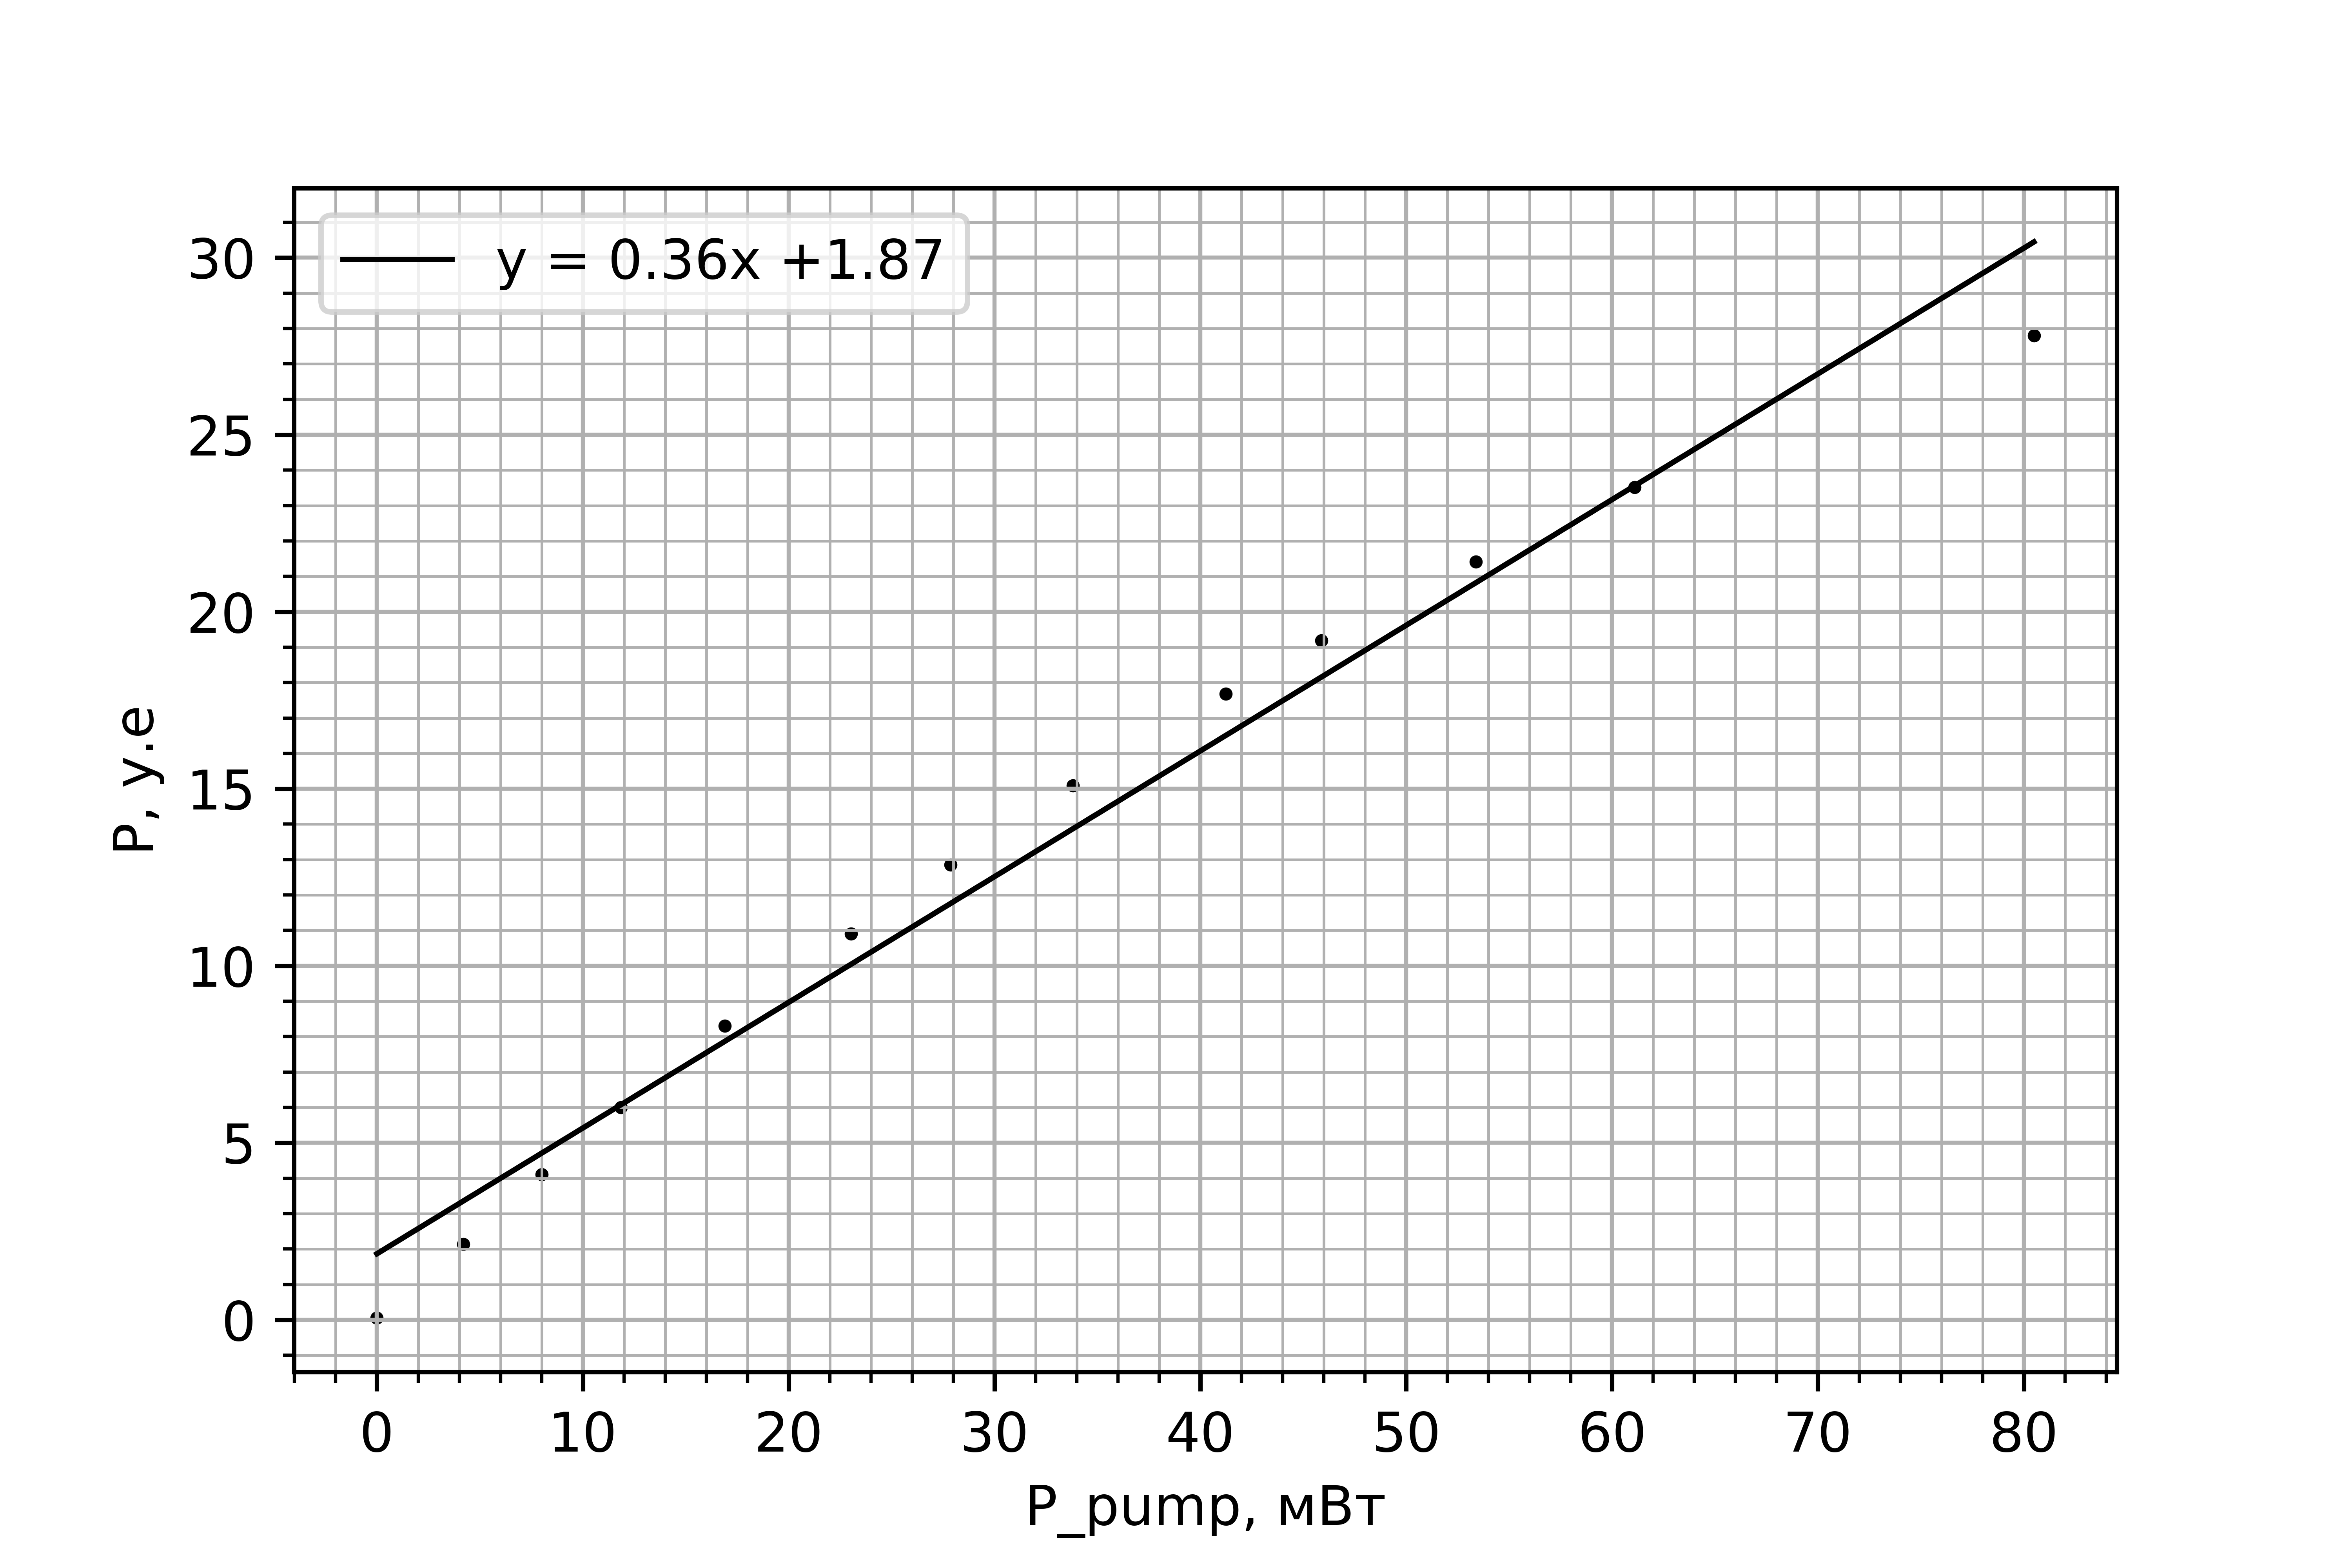
\includegraphics[scale=0.7]{Red_phdiod_1.png}
	\caption{Ватт-ваттная характеристика красного светодиода}
        \label{pic.1}
\end{figure}

\begin{figure}[H]
	\centering
	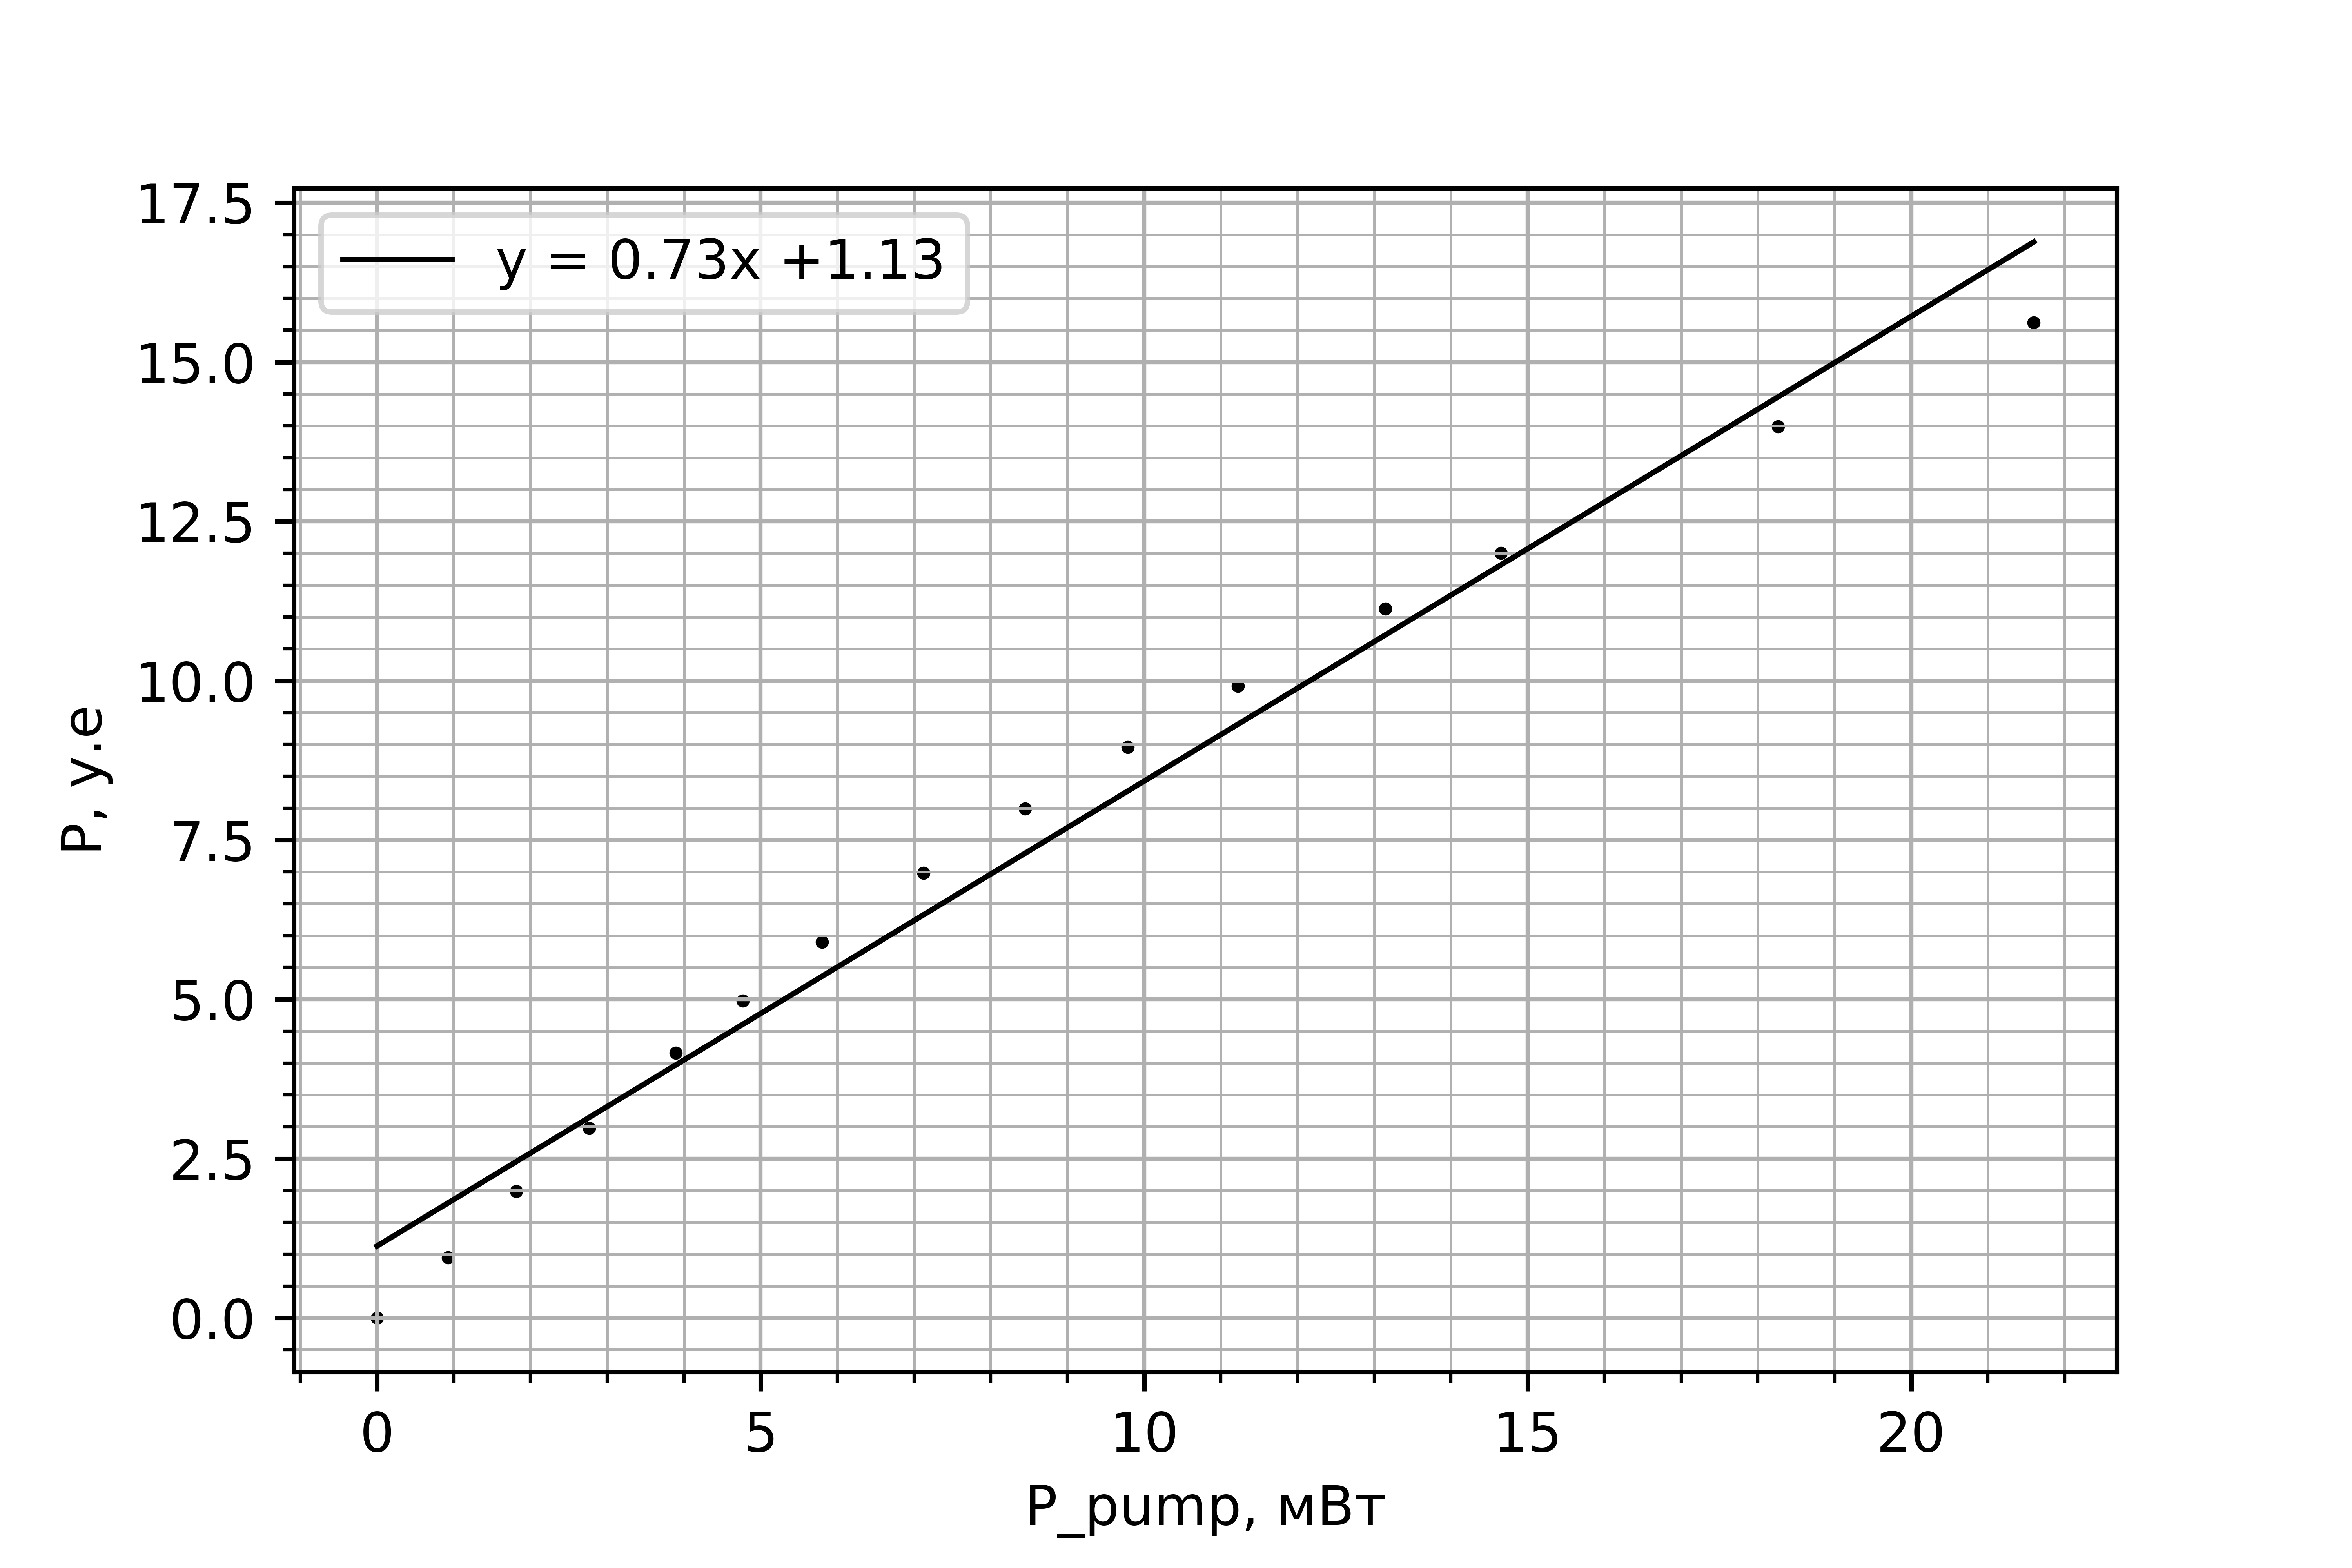
\includegraphics[scale=0.7]{Blue_phdiod_1.png}
	\caption{Ватт-ваттная характеристика синего светодиода}
        \label{pic.2}
\end{figure}

\begin{figure}[H]
	\centering
	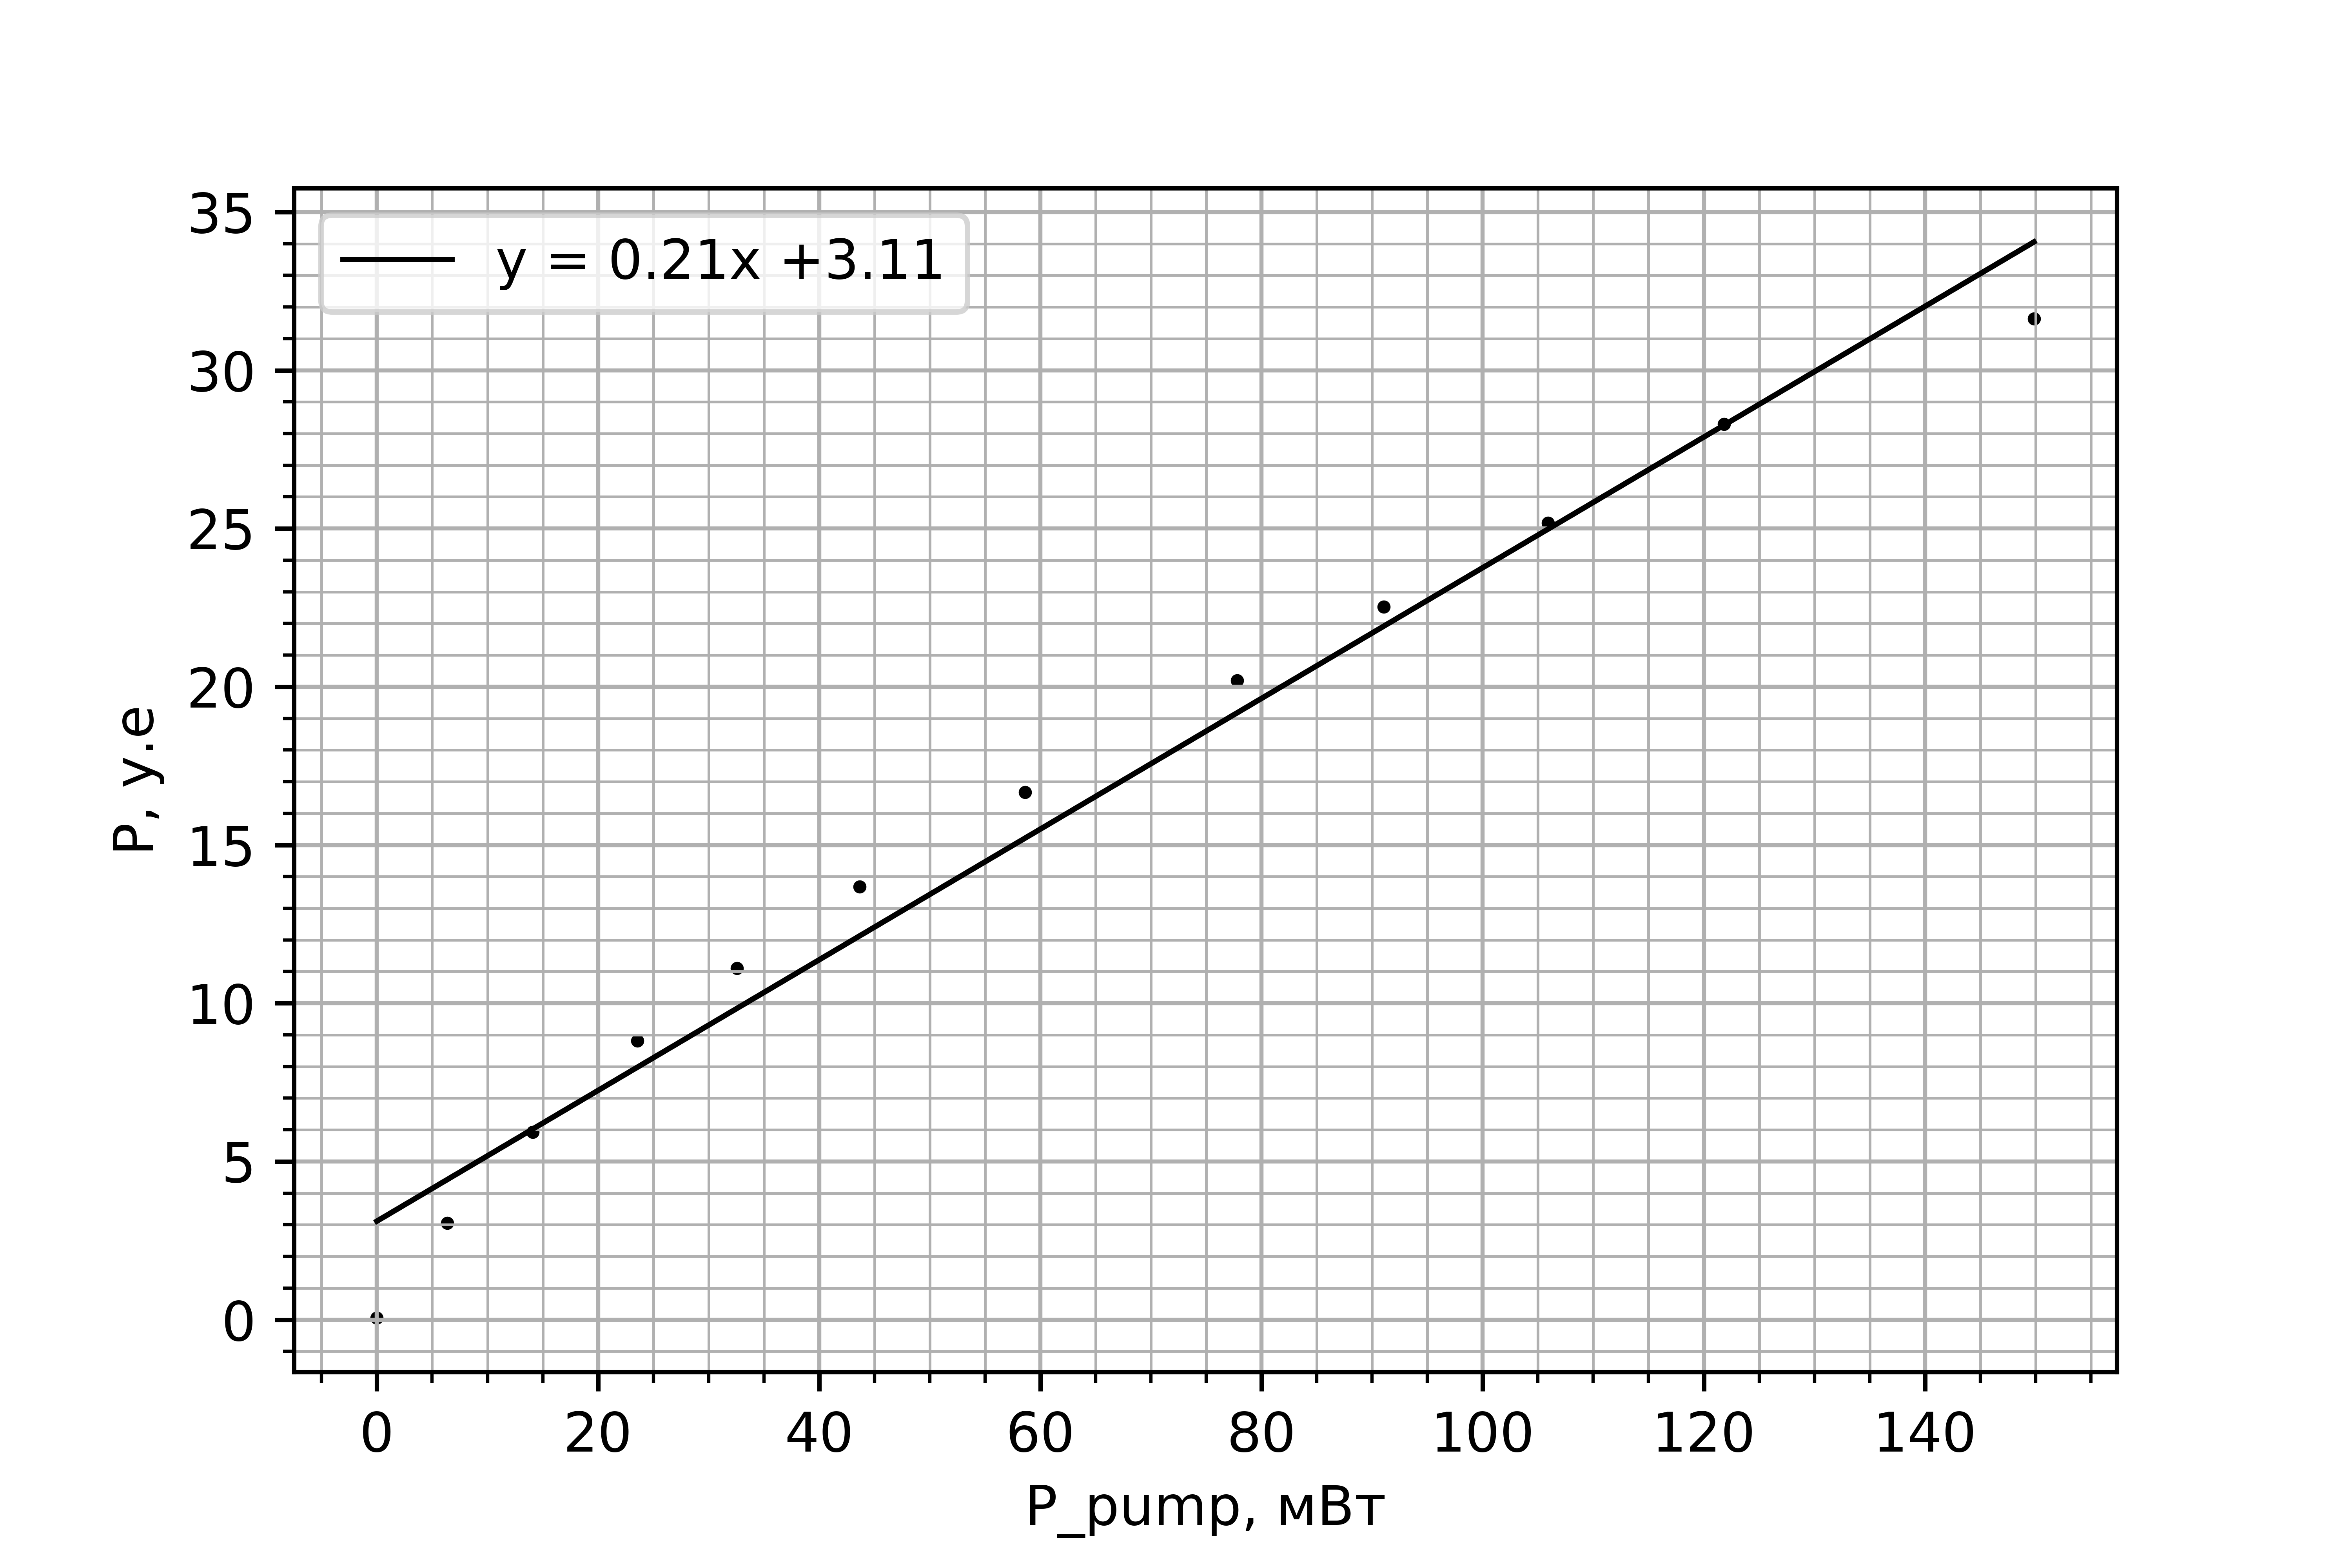
\includegraphics[scale=0.7]{Green_phdiod_1.png}
	\caption{Ватт-ваттная характеристика зеленого светодиода}
        \label{pic.3}
\end{figure}

\begin{figure}[H]
	\centering
	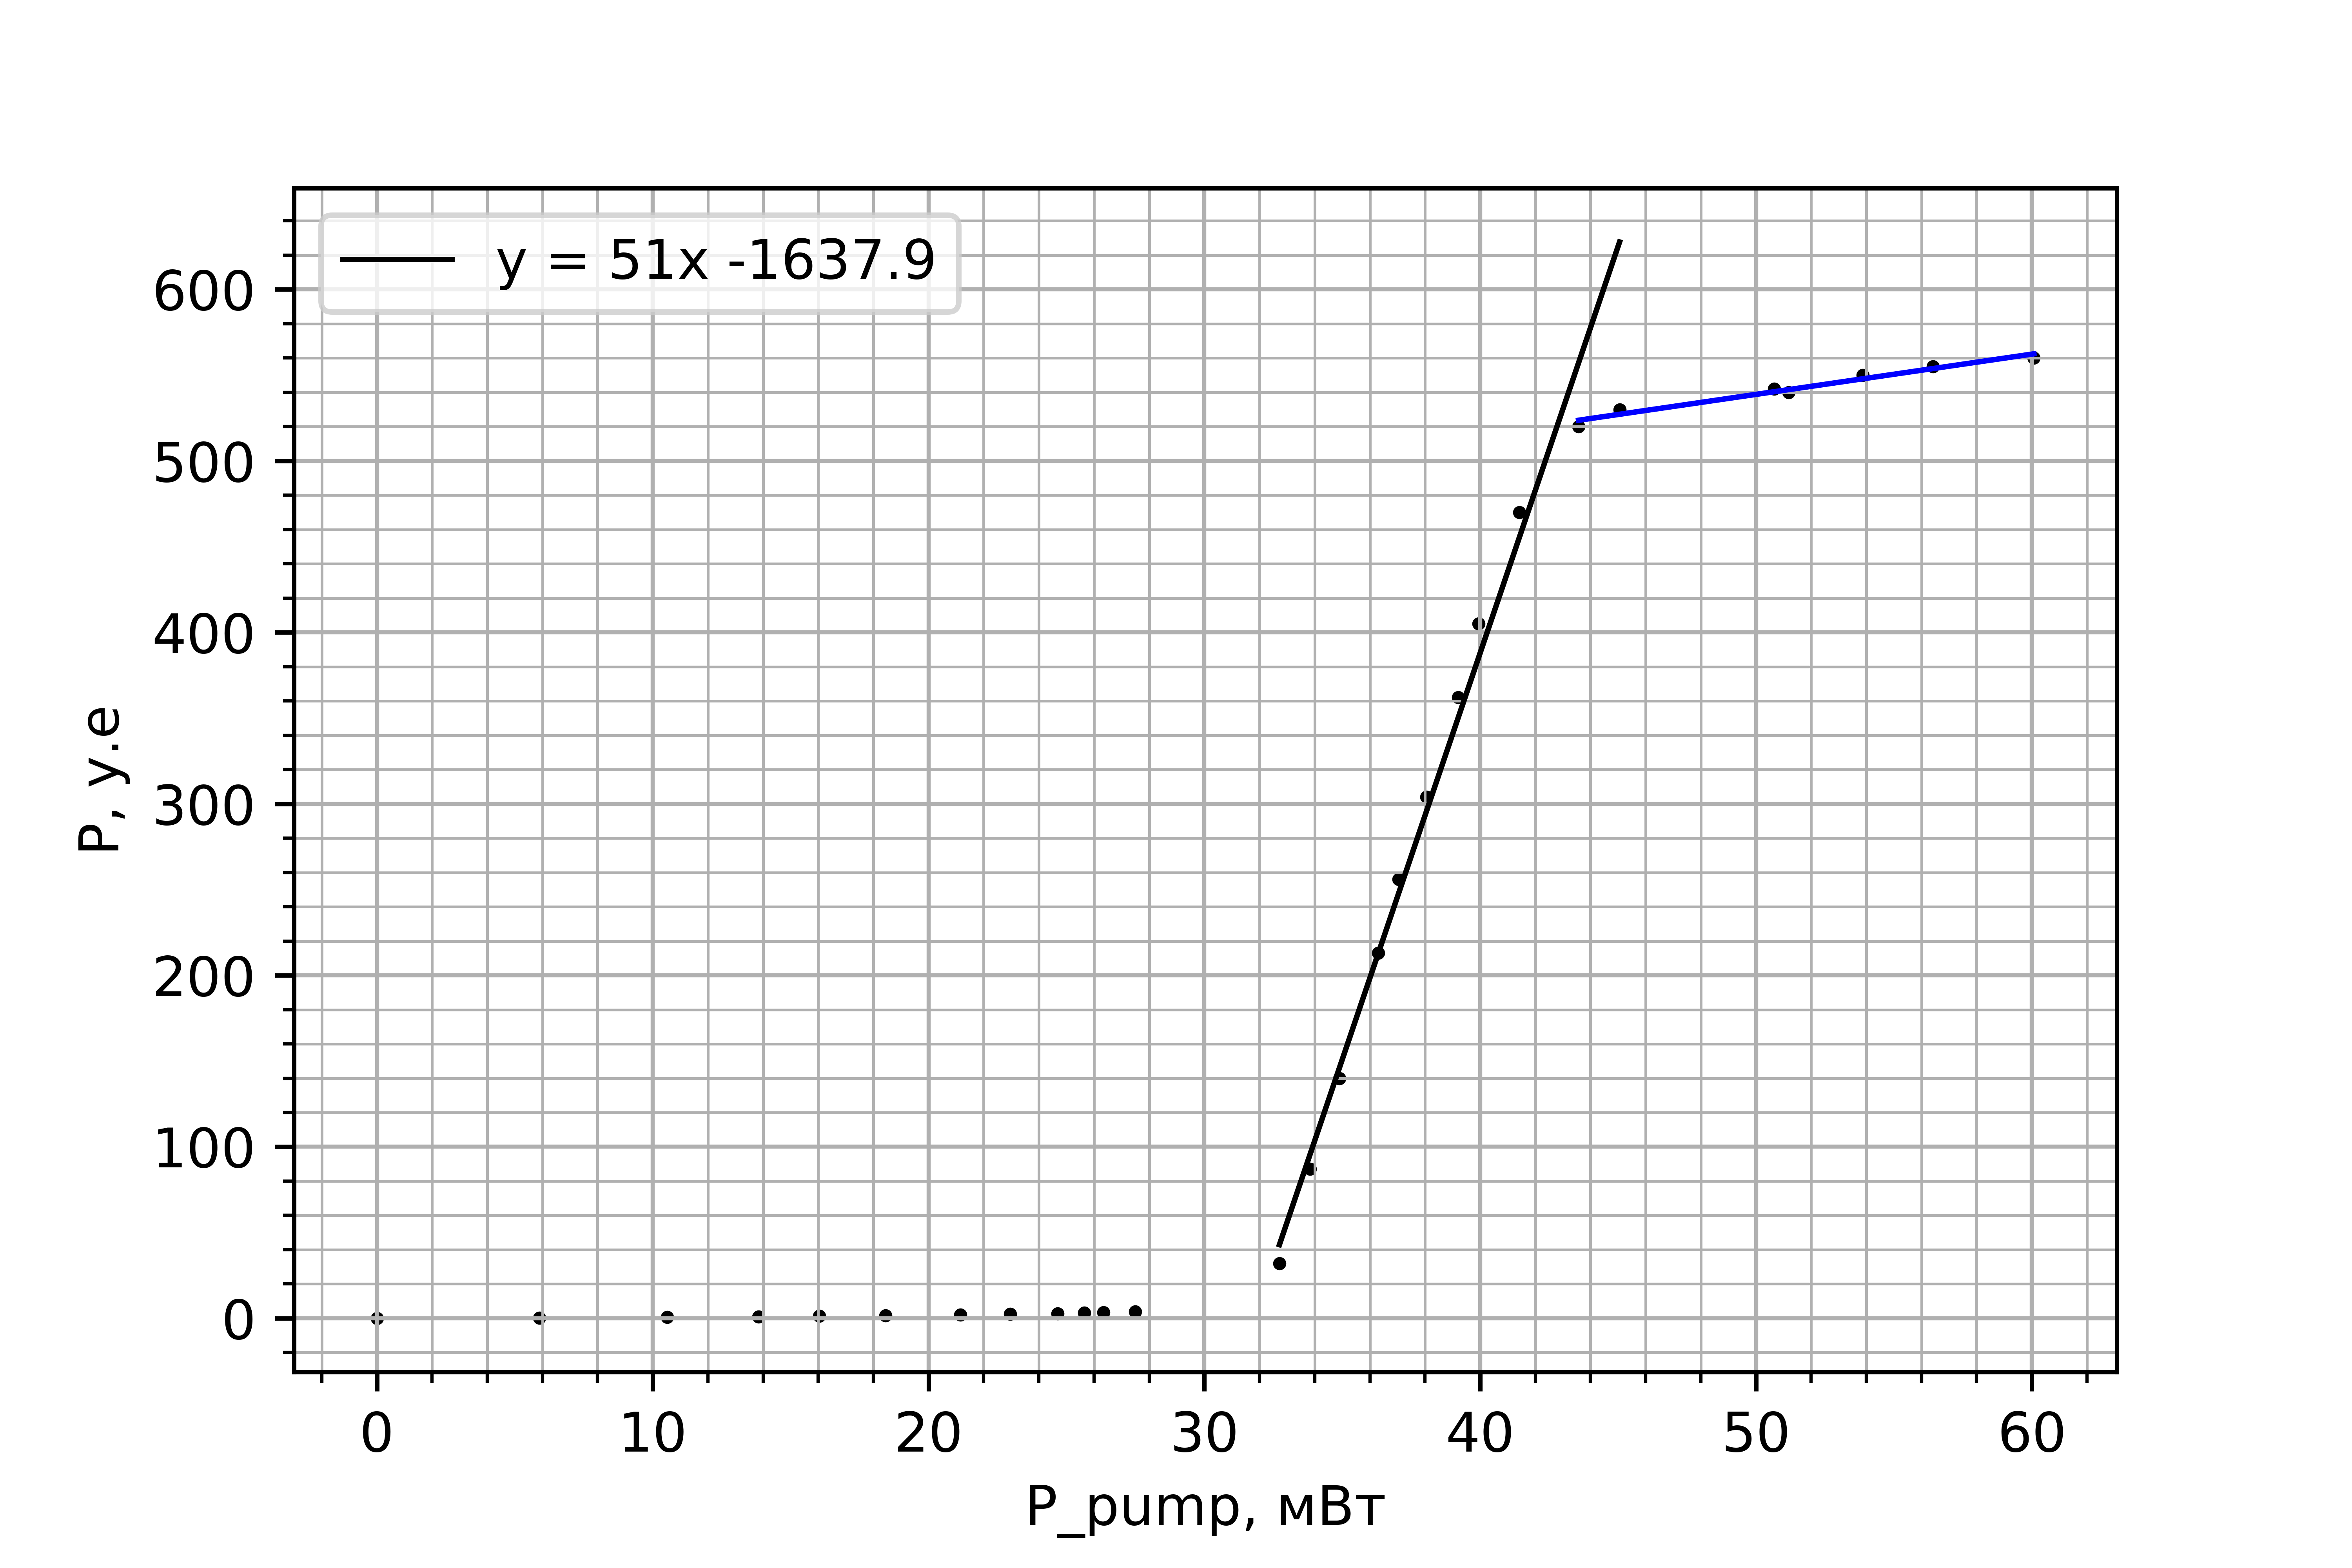
\includegraphics[scale=0.7]{Red_lazer_1.png}
	\caption{Ватт-ваттная характеристика красного лазера}
        \label{pic.4}
\end{figure}

Используя ватт-ваттную характеристику красного лазера, найдем пороговую мощность $P_{\text{порог}}$ и мощность насыщения $P_{\text{нас}}$:
\begin{center}
    $P_{\text{порог}} = 31,8$ мВт, $P_{\text{нас}} = 42,8$ мВт
\end{center}

\subsection*{2. Спектральные характеристики}

Используя полученные данные (см. таблица \ref{tab.6}-\ref{tab.11}),исследуем зависимость спектра излучения инжекционного полупроводникового лазера и светодиодов от мощности накачки производится, измерив детектируемую длину волны и фиксируя напряжения при постоянной мощности накачки (см. рис.\ref{pic.5}-\ref{pic.9}). Ширина линии и центральная длина волны указаны в таблице \ref{tab.1}.

\begin{figure}[H]
	\centering
	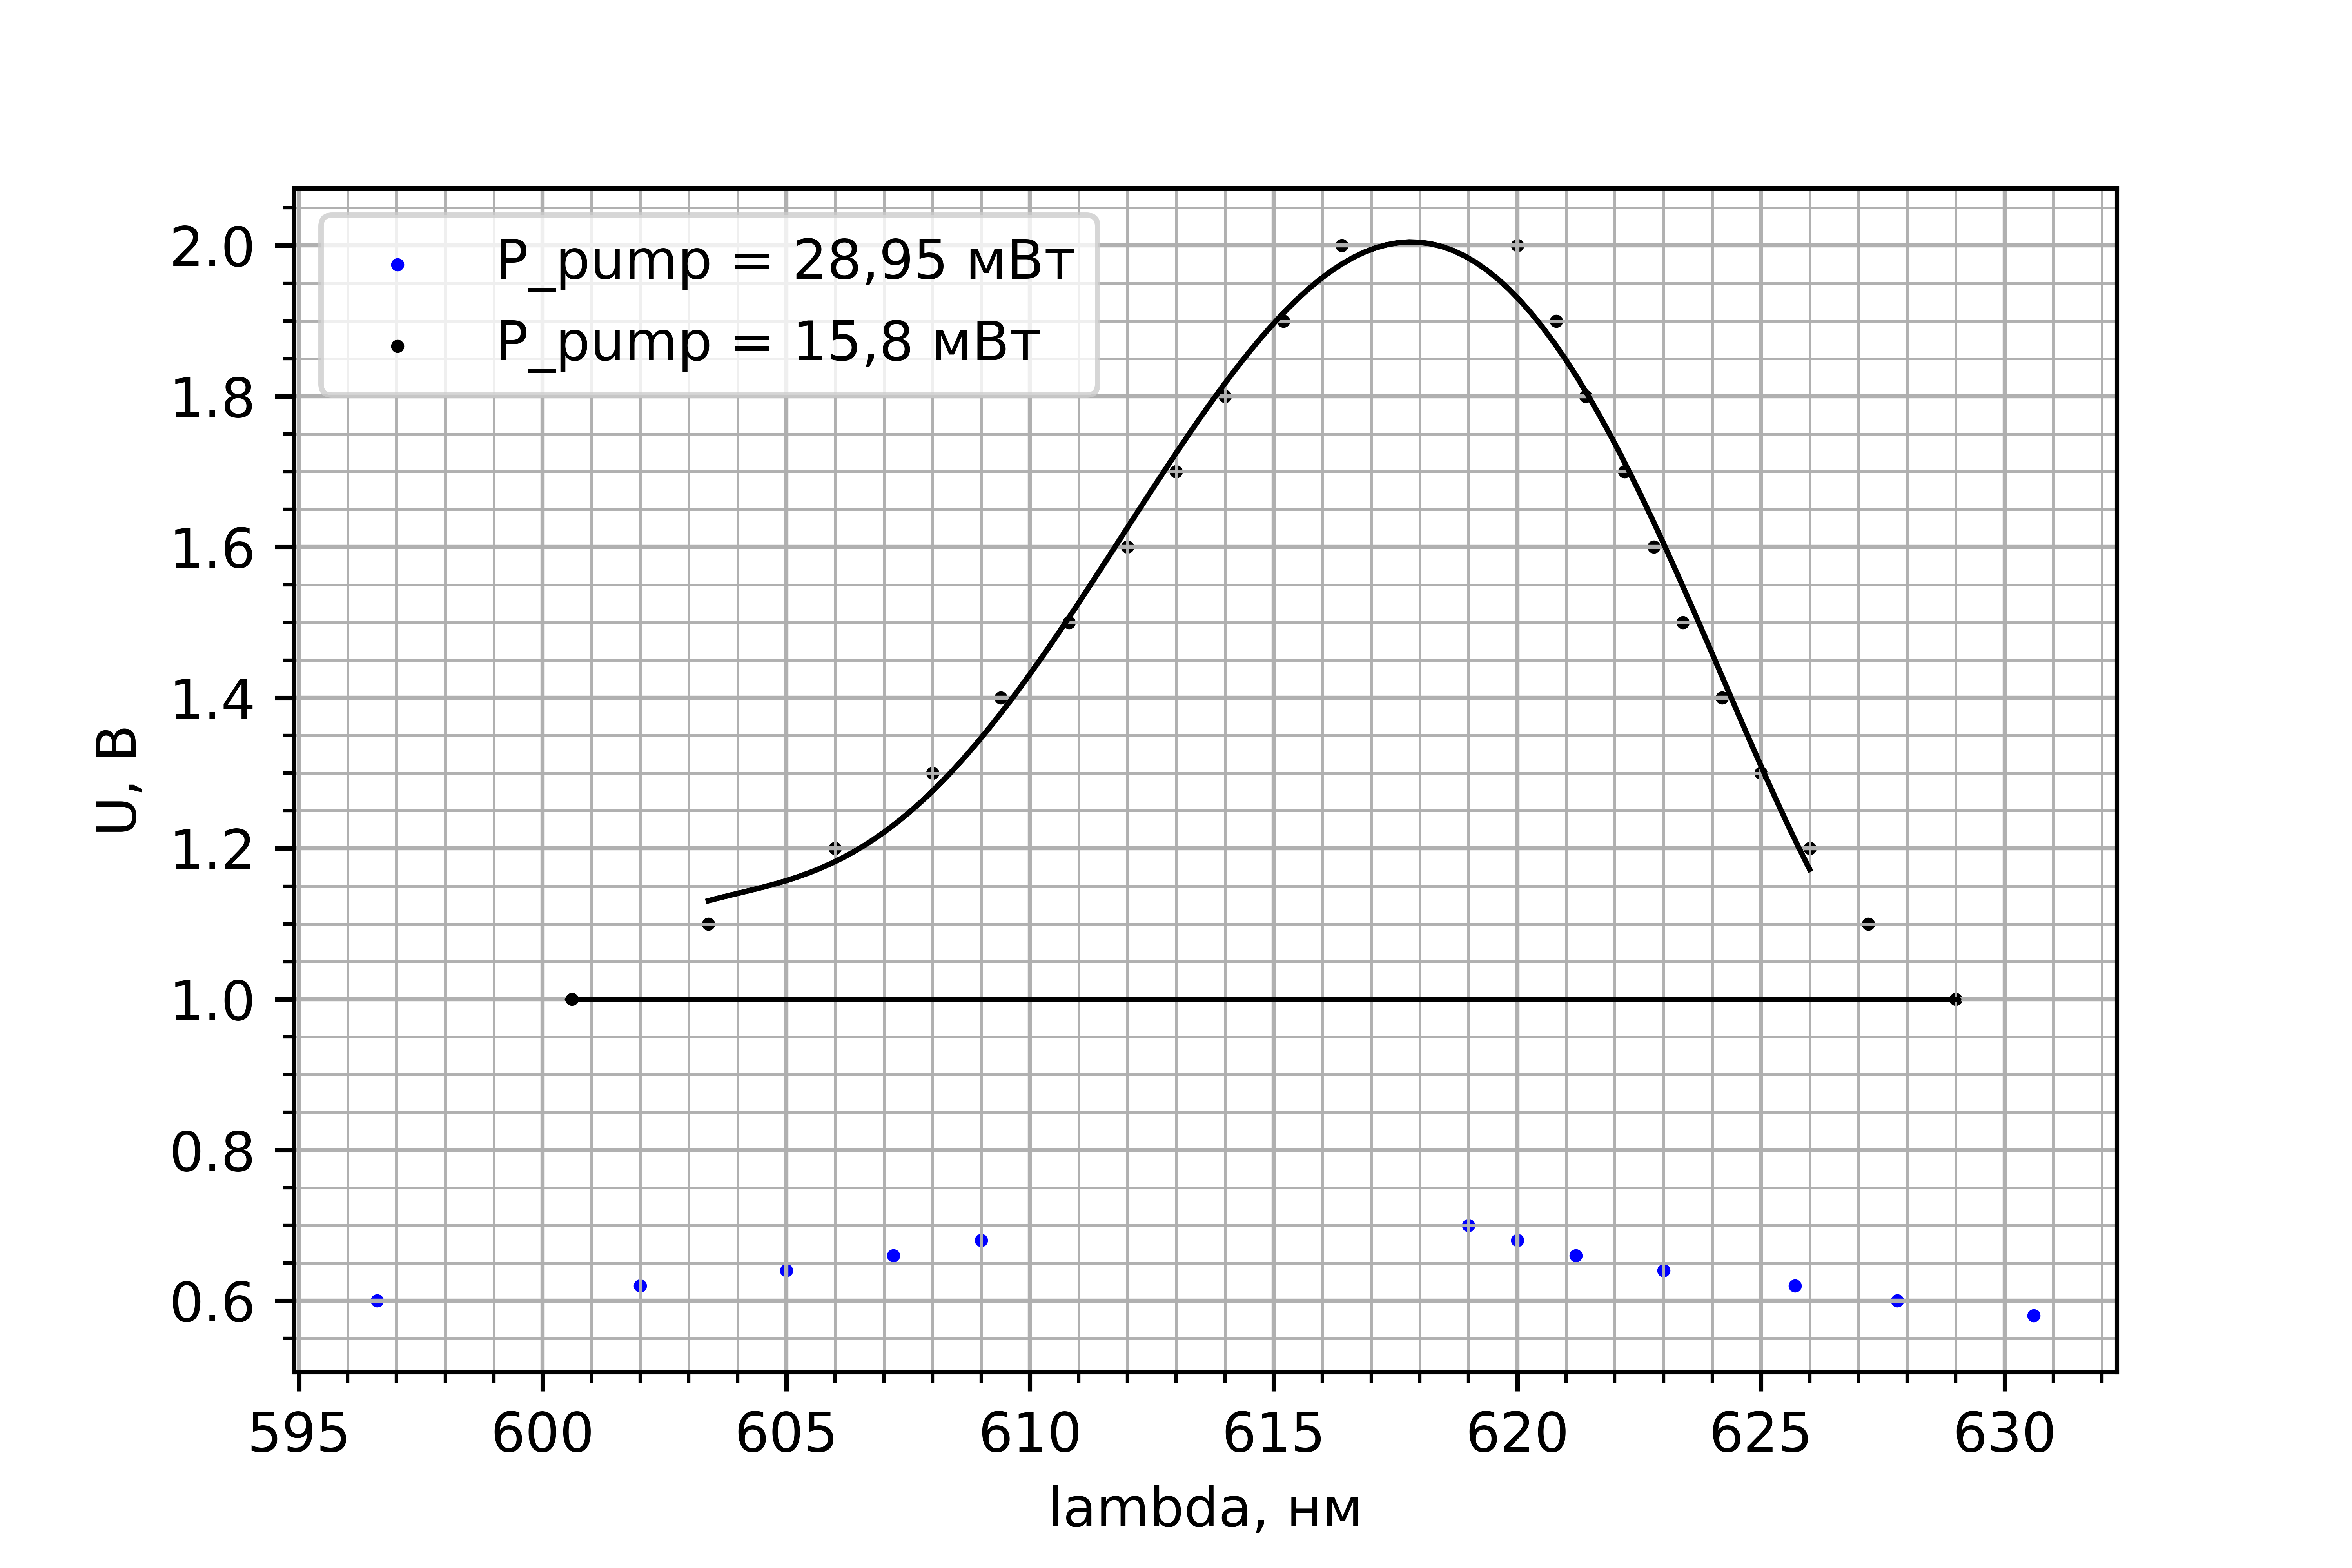
\includegraphics[scale=0.7]{Red_phdiod_2.png}
	\caption{Спектральная характеристика красного светодиода}
        \label{pic.5}
\end{figure}

\begin{figure}[H]
	\centering
	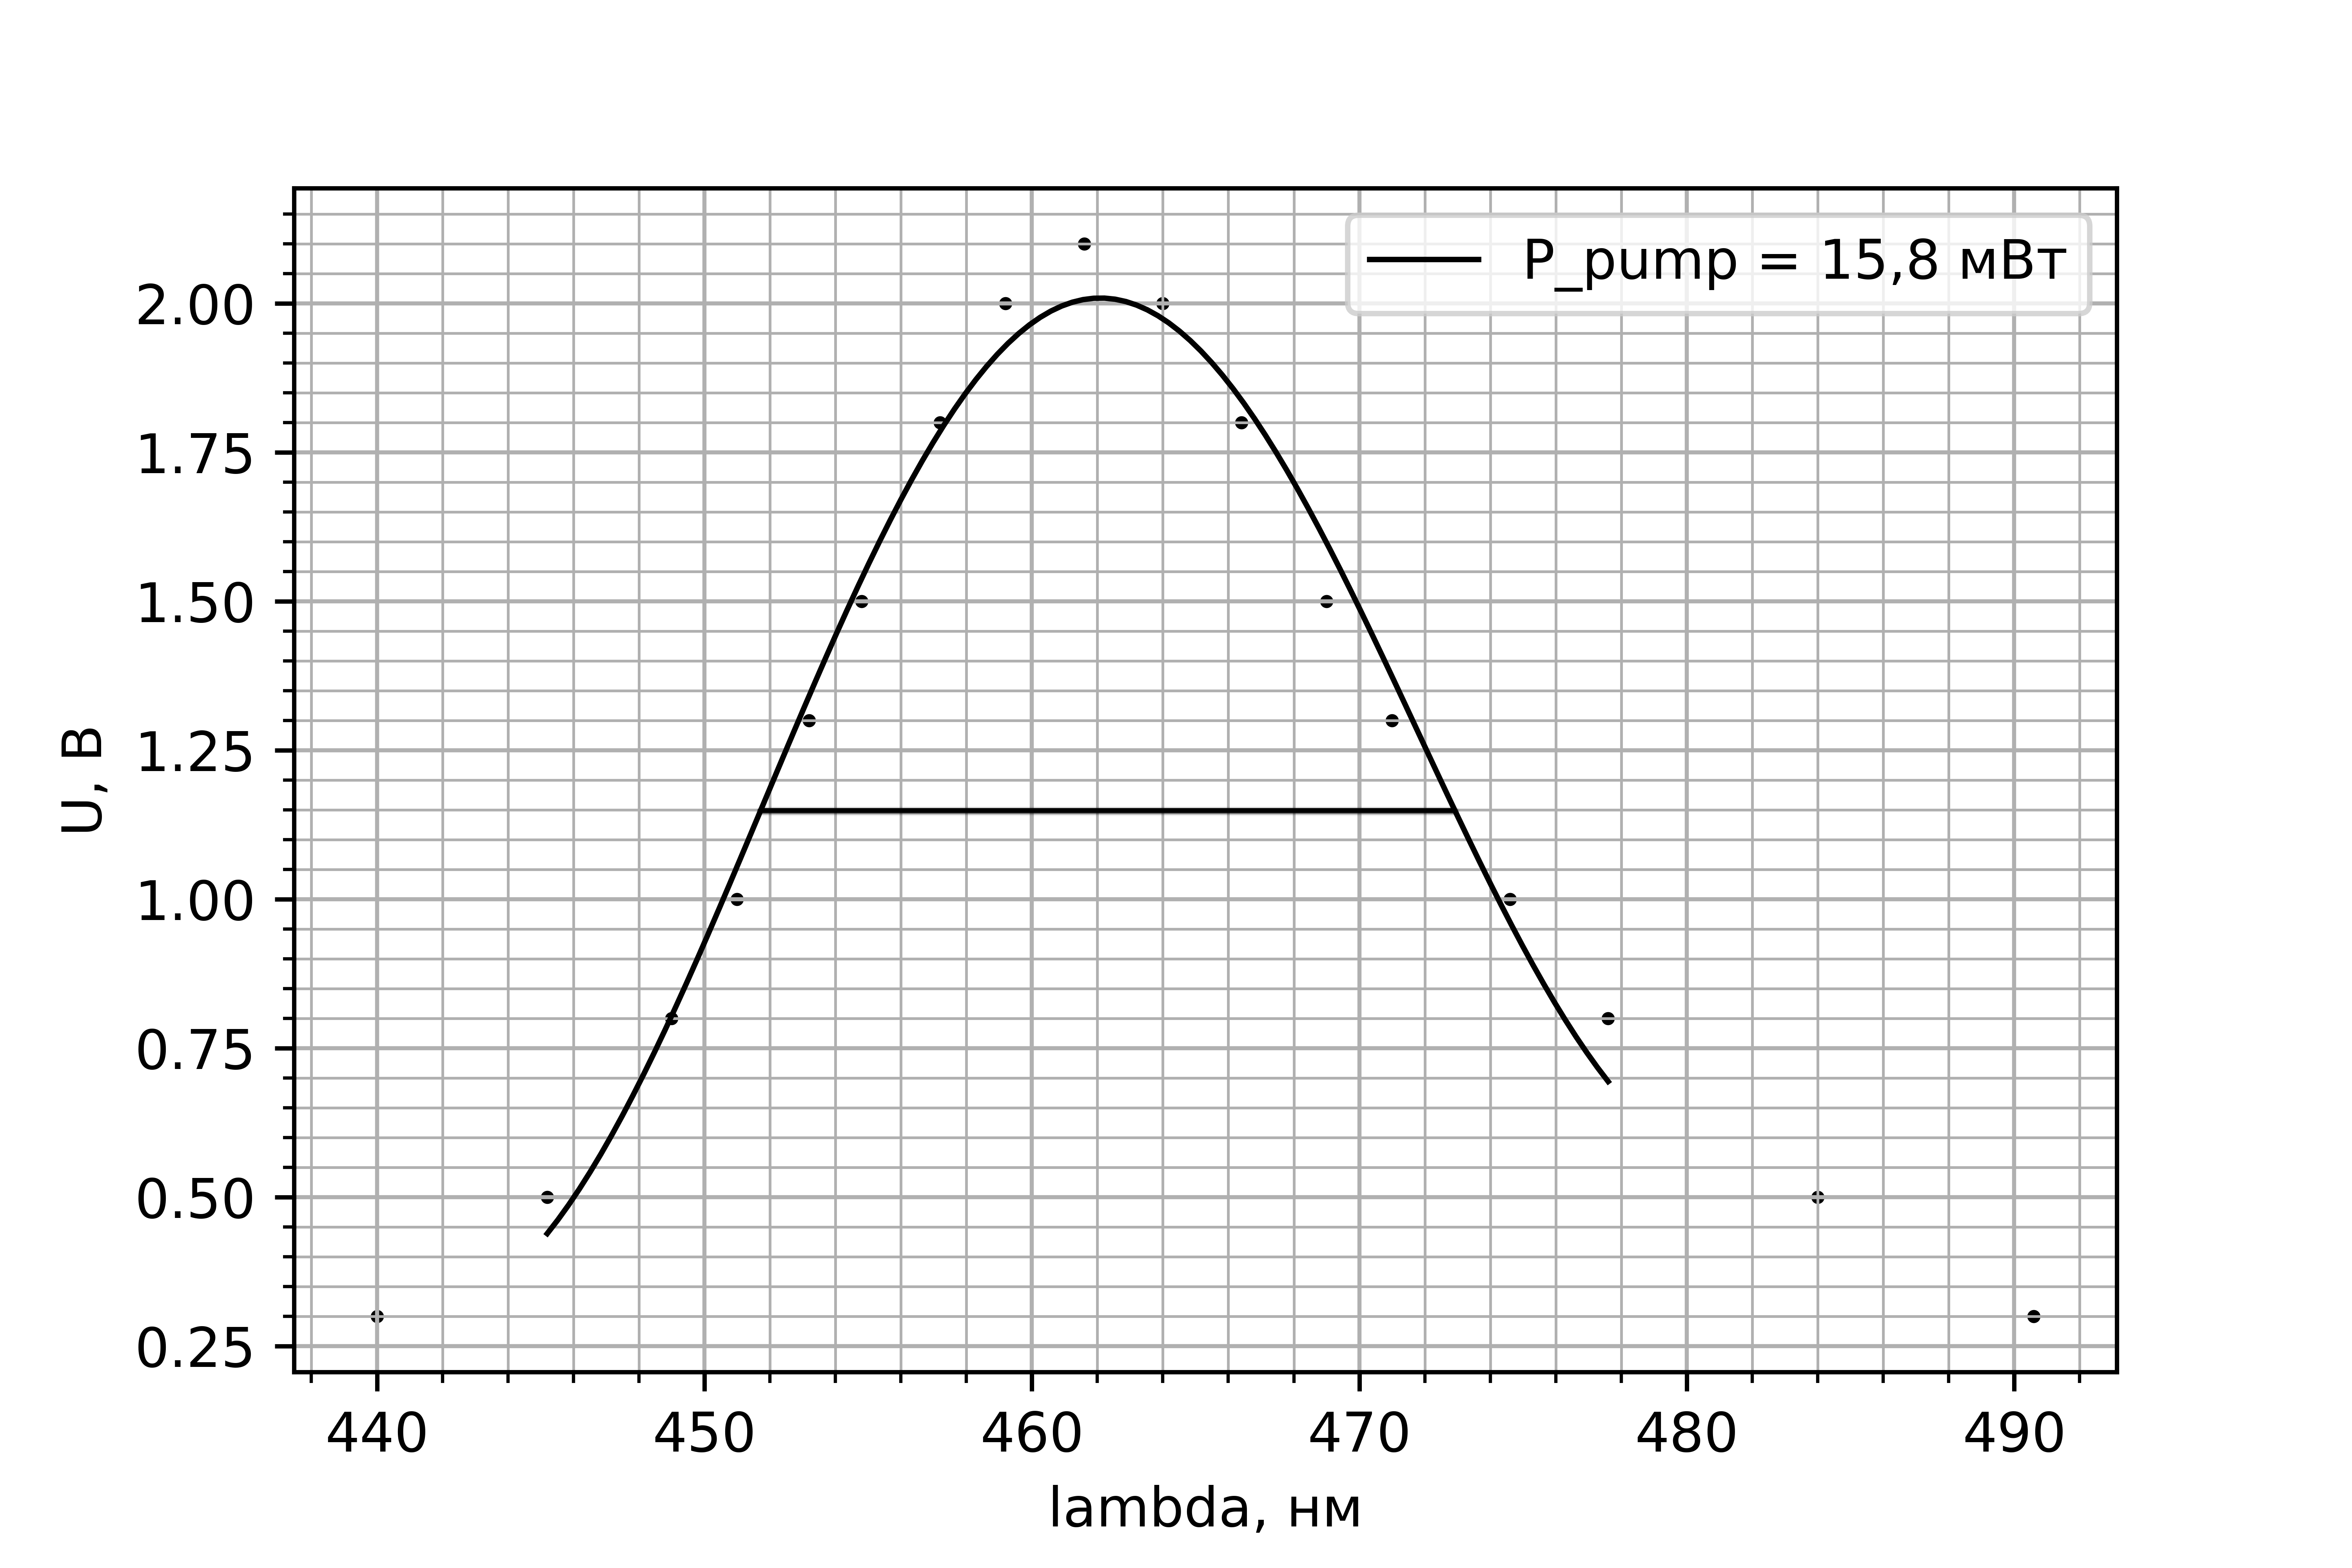
\includegraphics[scale=0.7]{Blue_phdiod_2.png}
	\caption{Спектральная характеристика синего светодиода}
        \label{pic.6}
\end{figure}

\begin{figure}[H]
	\centering
	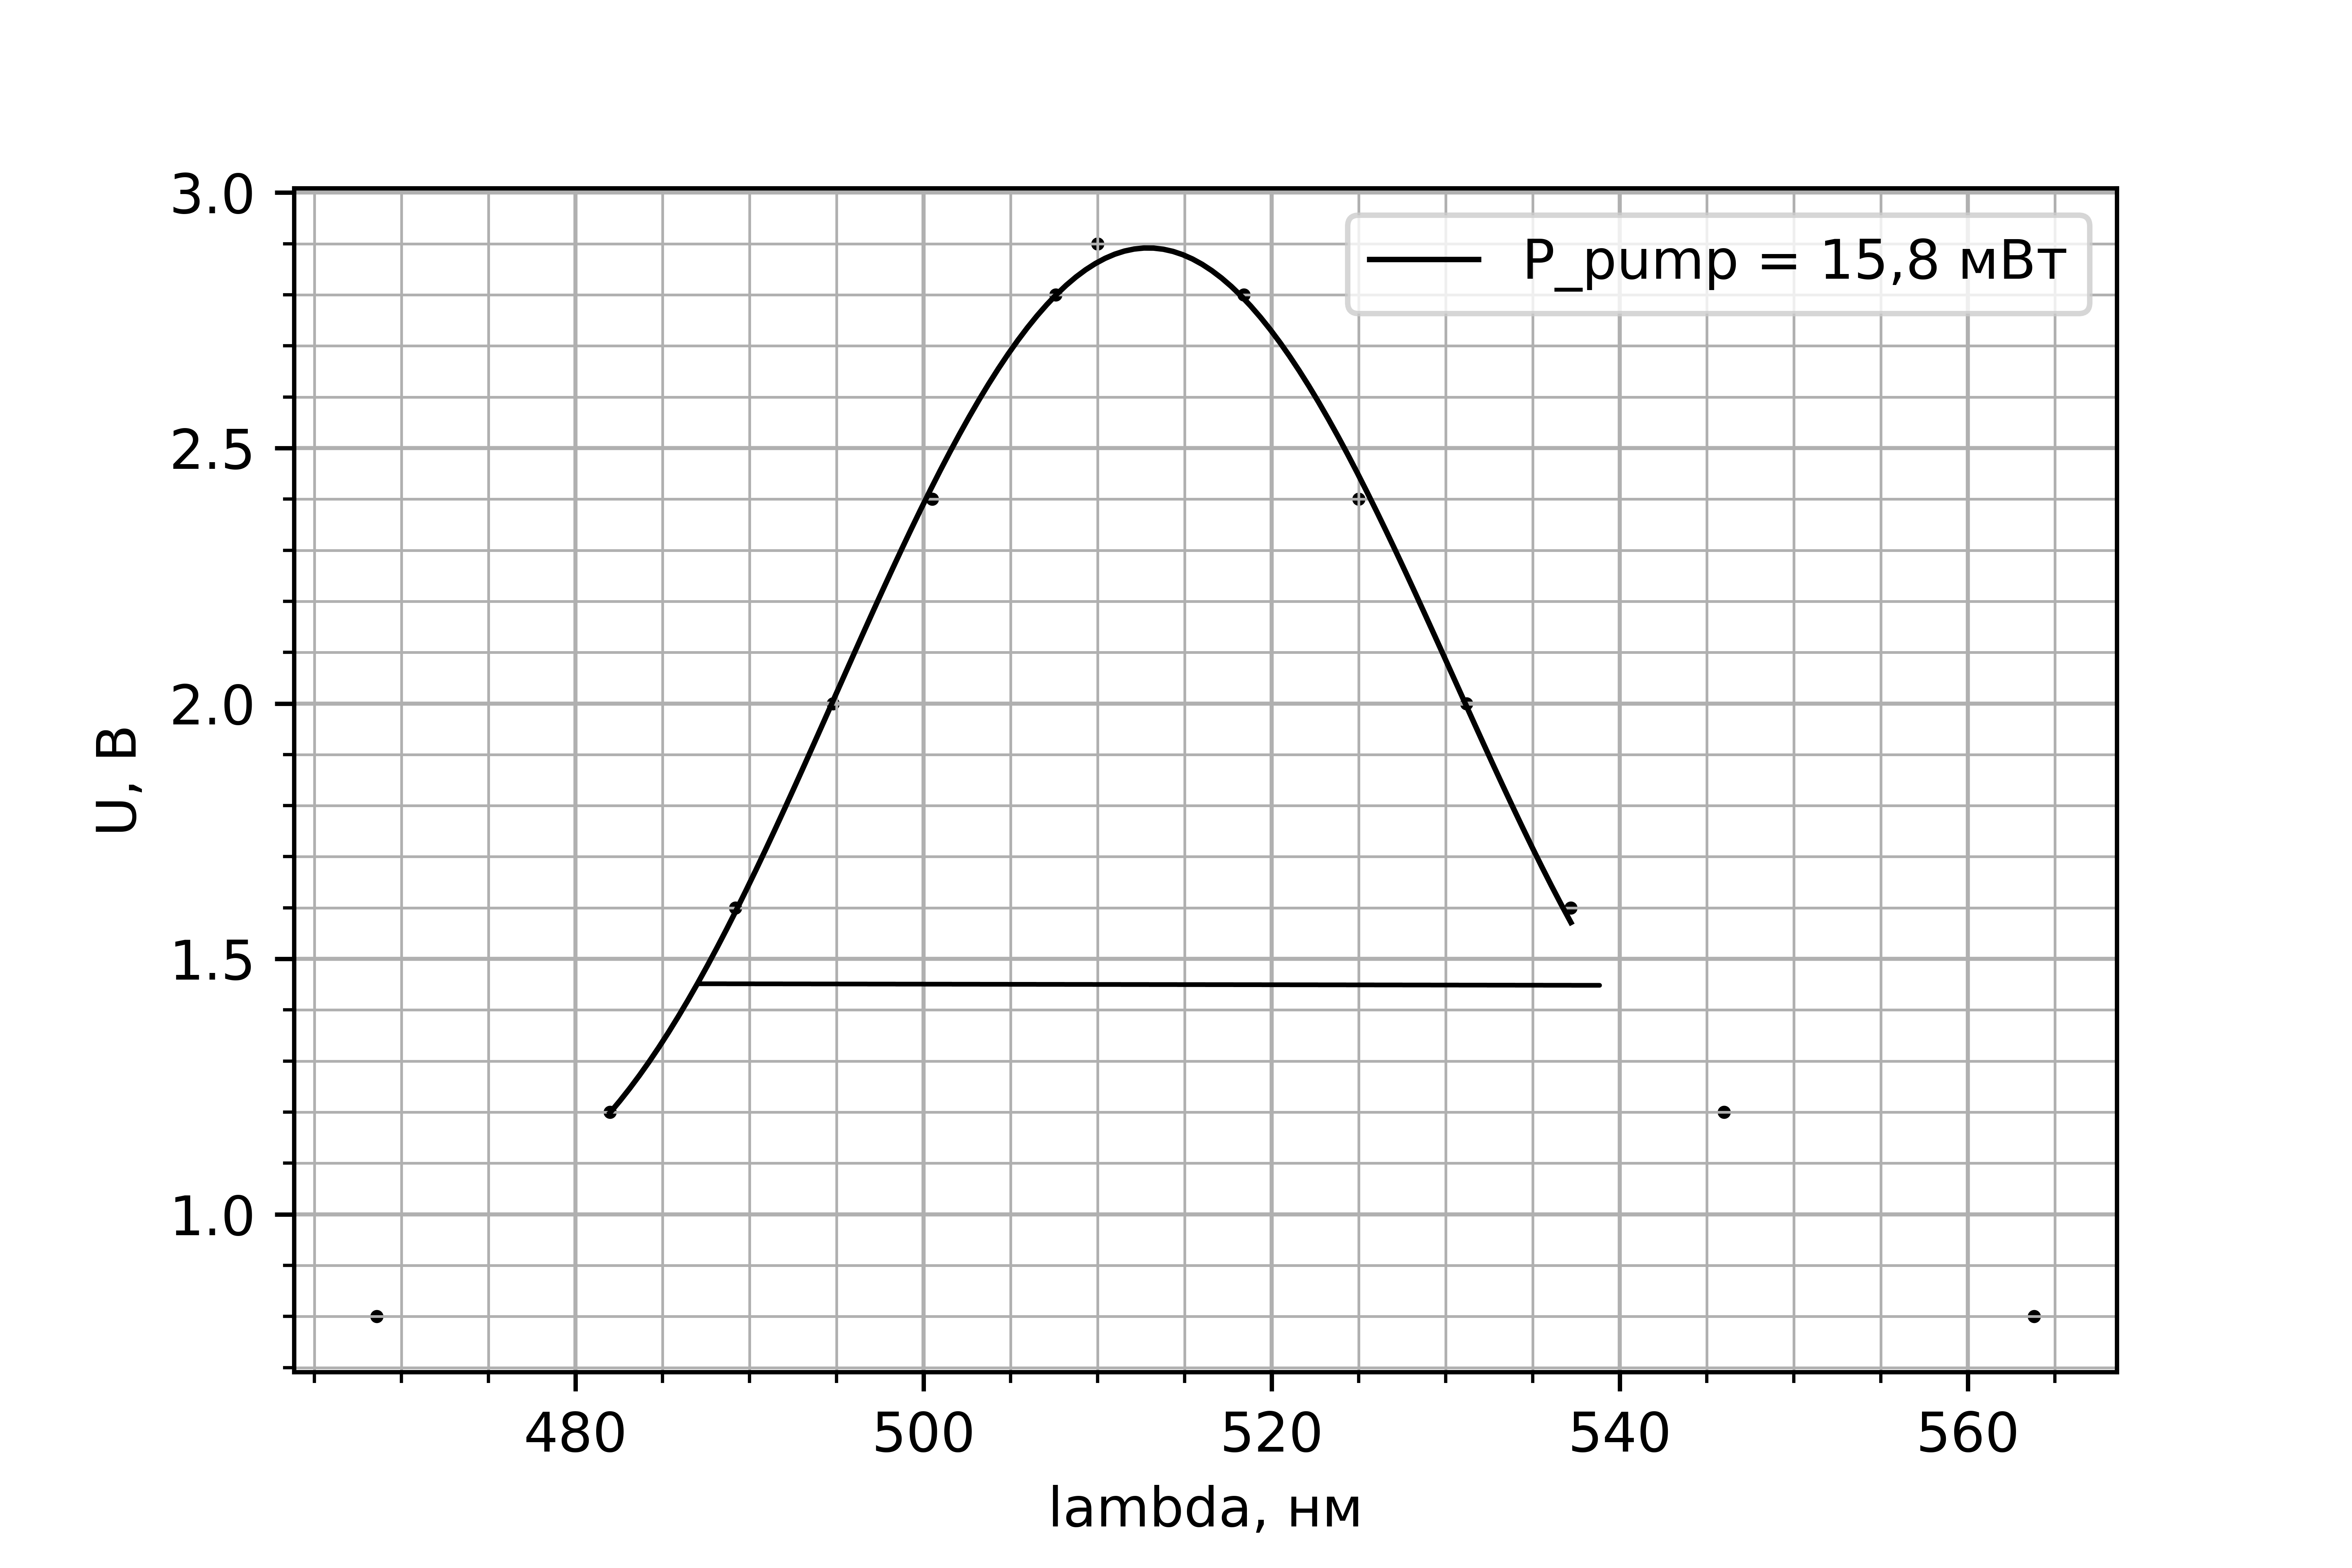
\includegraphics[scale=0.7]{Green_phdiod_2.png}
	\caption{Спектральная характеристика зеленого светодиода}
        \label{pic.7}
\end{figure}

\begin{figure}[H]
	\centering
	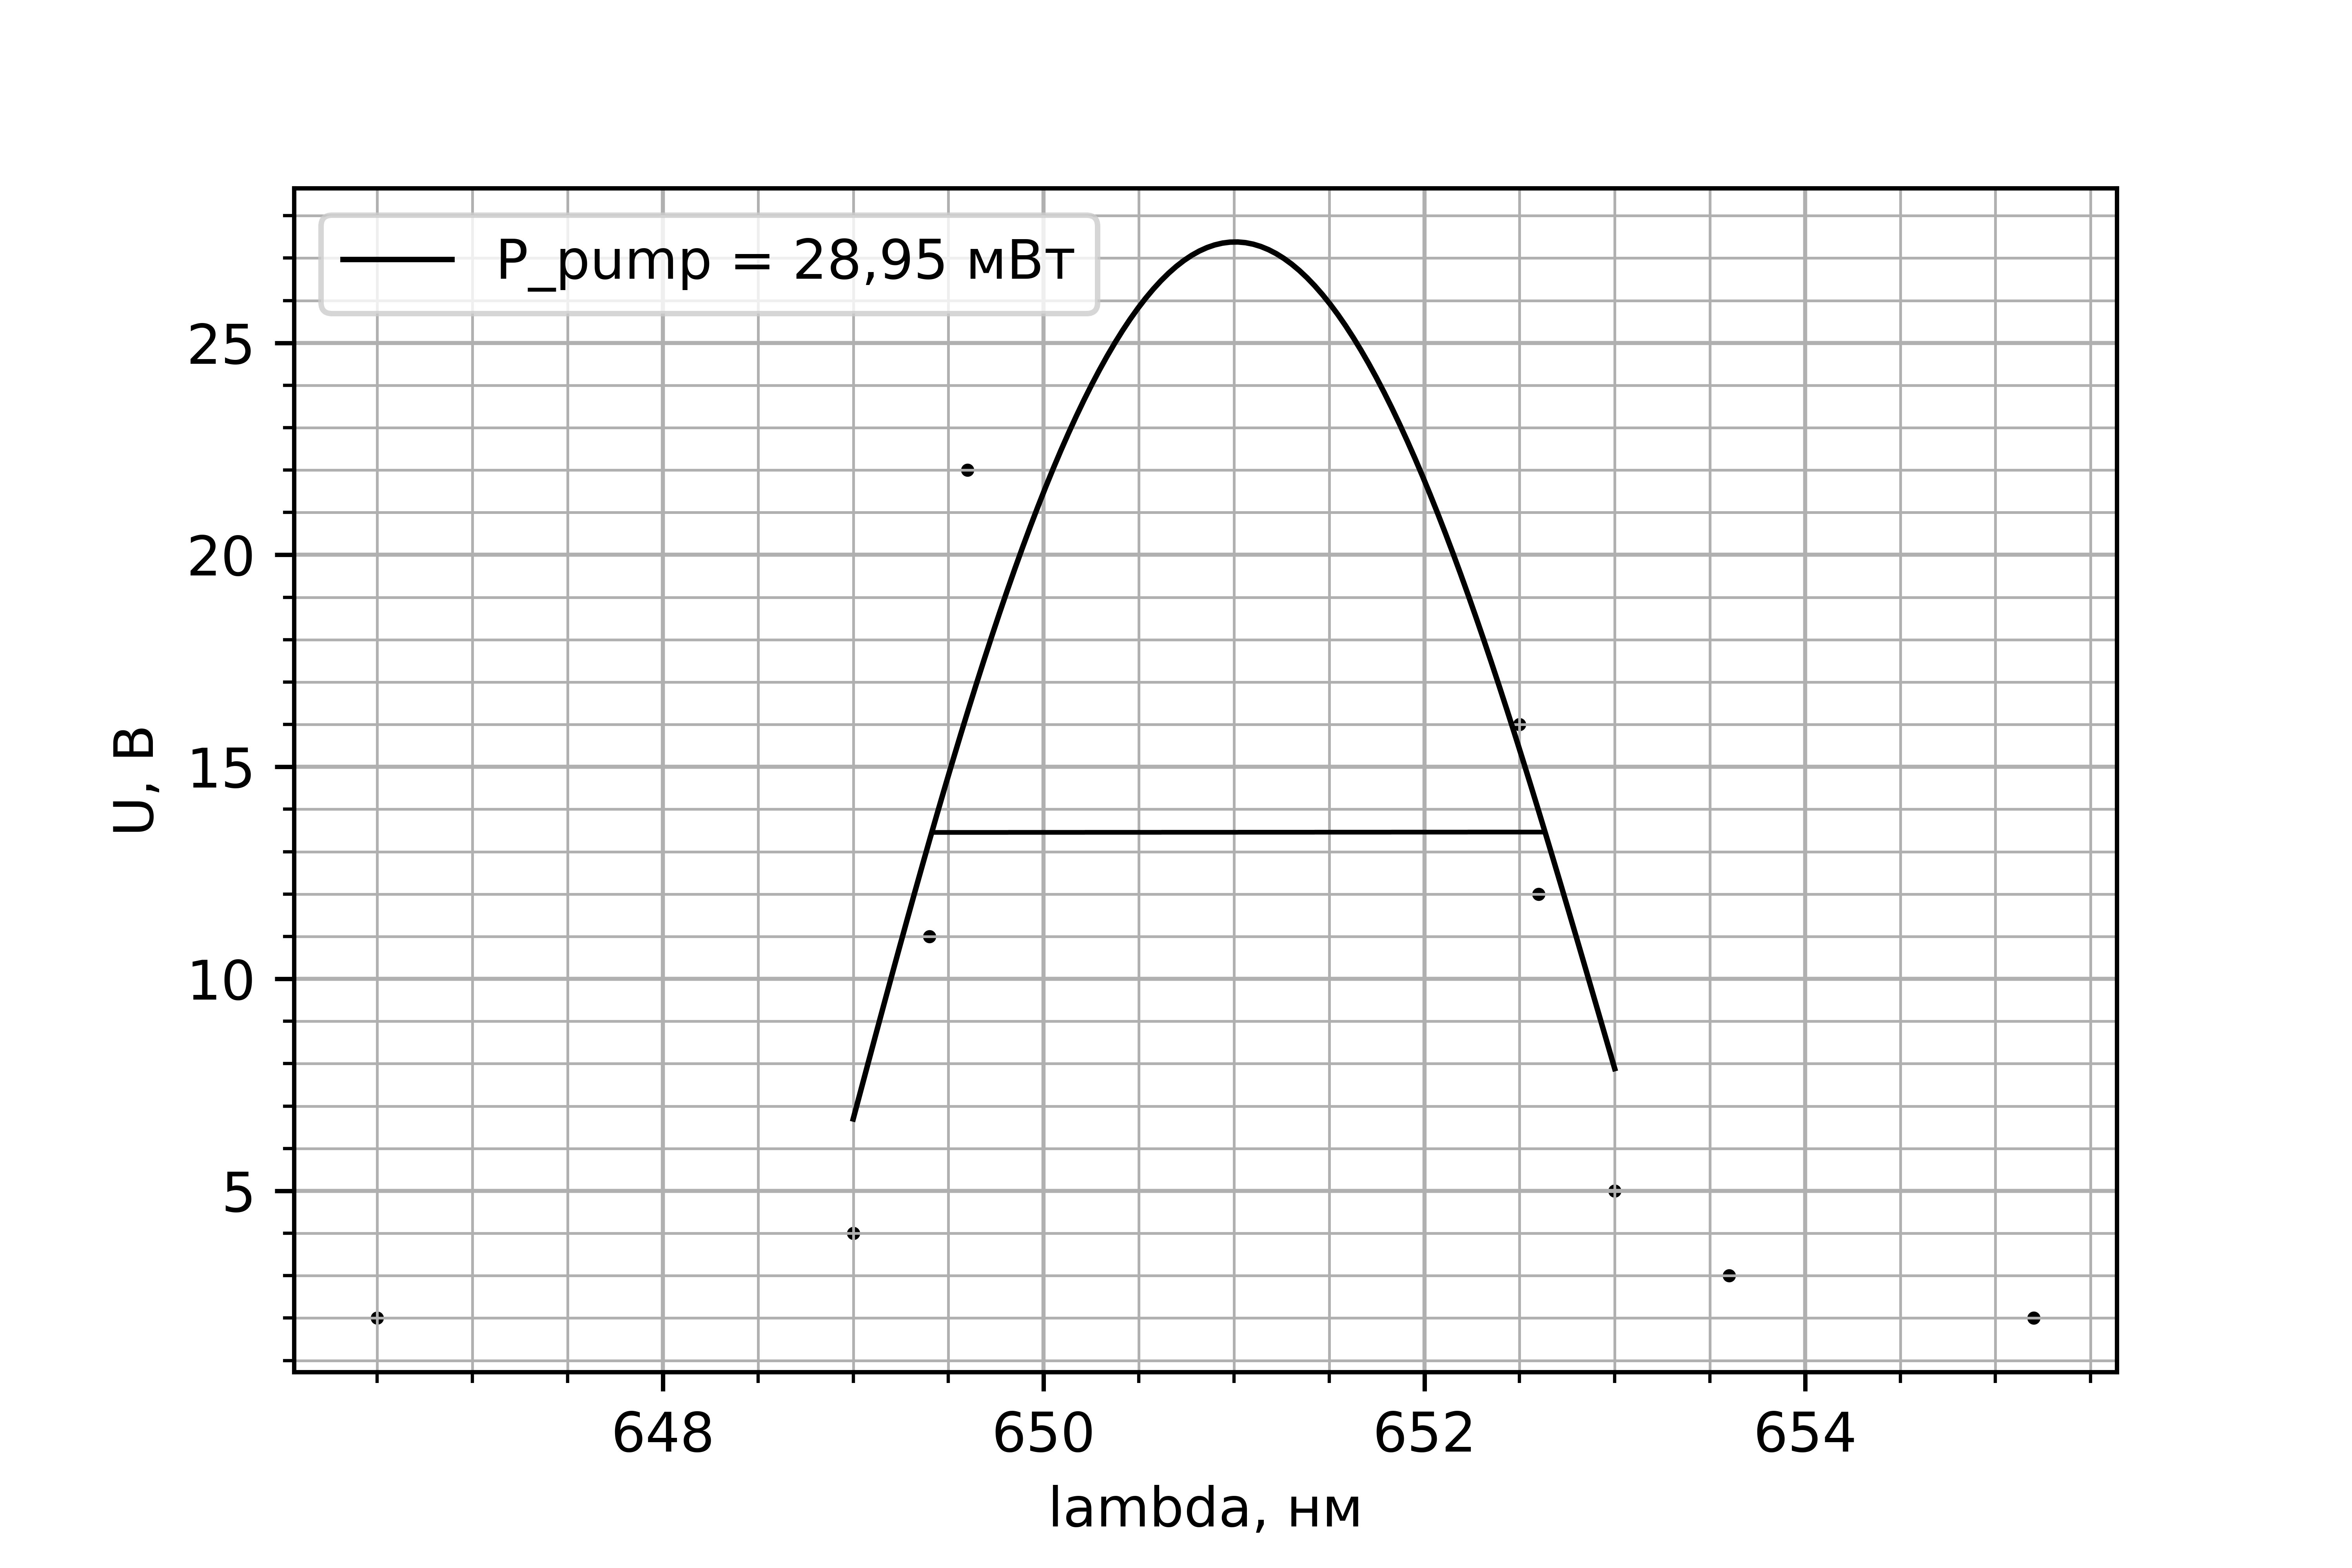
\includegraphics[scale=0.7]{Red_lazer_2_P_pump = 28,95.png}
	\caption{Спектральная характеристика красного лазера при $P_{pump} = 28,95$ мВт}
        \label{pic.8}
\end{figure}

\begin{figure}[H]
	\centering
	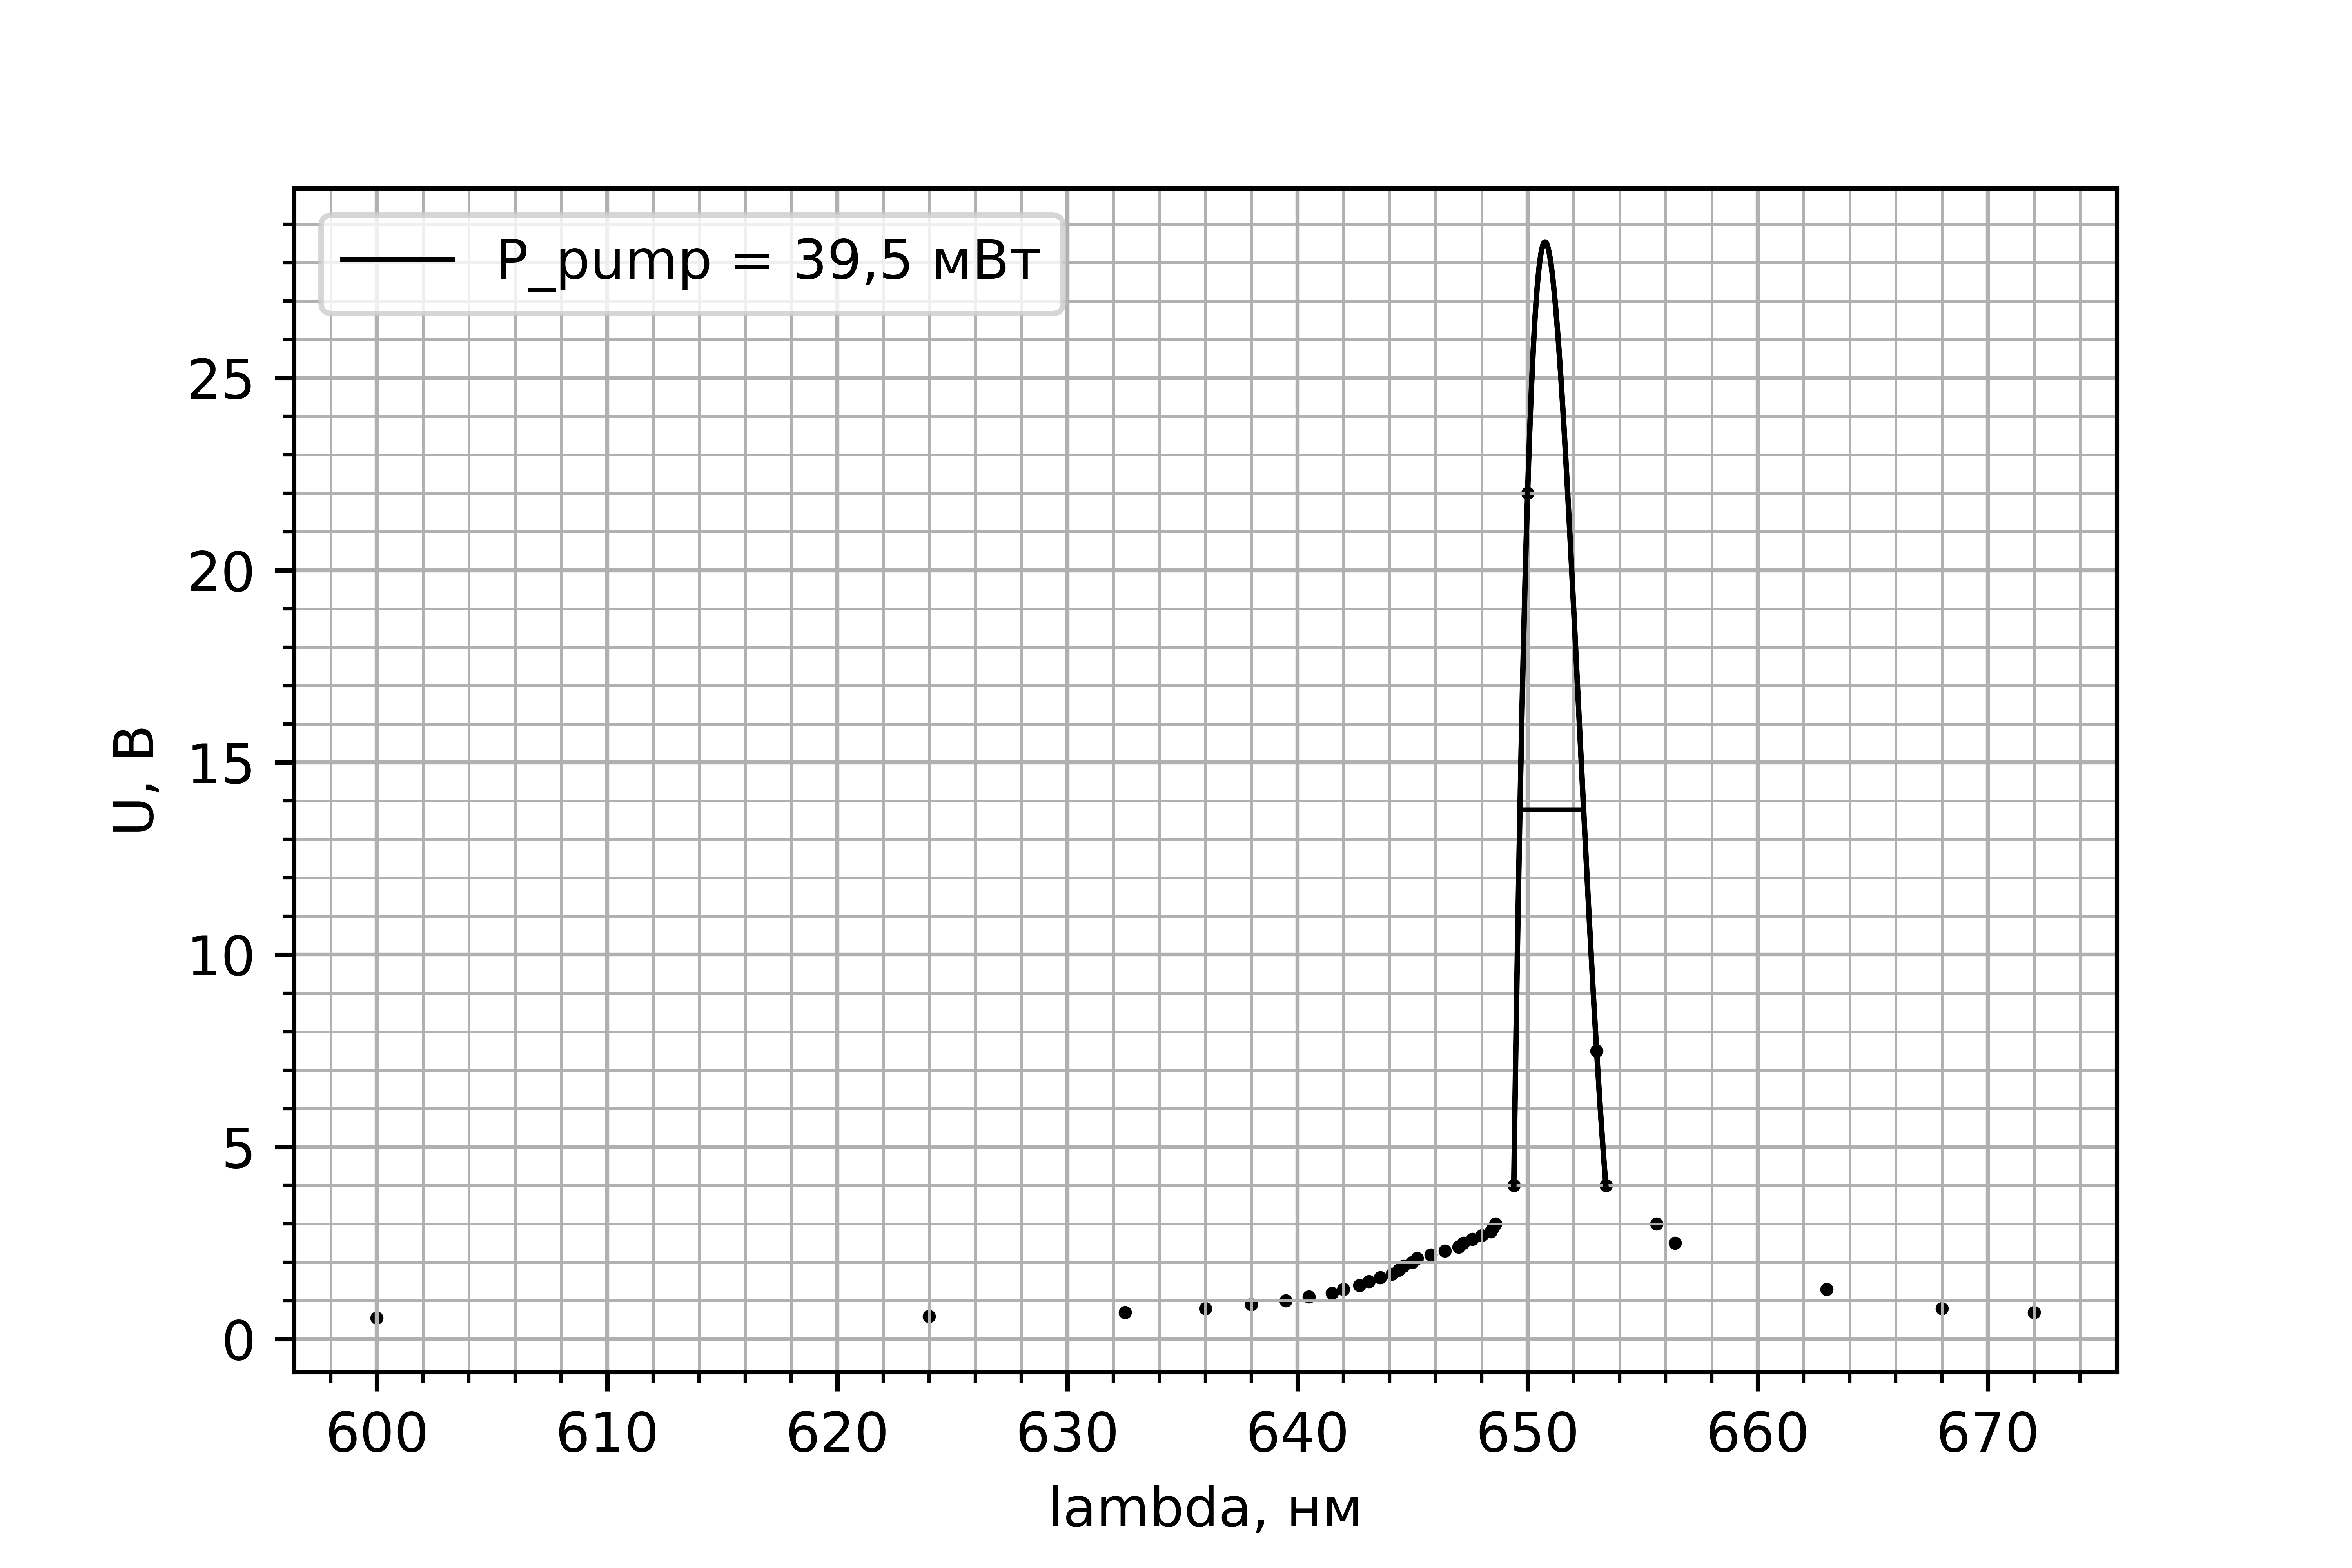
\includegraphics[scale=0.7]{Red_lazer_2_P_pump = 39,5.png}
	\caption{Спектральная характеристика красного лазера при $P_{pump} = 39,5$ мВт}
        \label{pic.9}
\end{figure}

\begin{table}[H]
\begin{tabular}{|c|c|c|}
\hline
                                     & $\lambda_{peak}$, нм & $\Delta\lambda$, нм \\ \hline
Красный лазер, $P_{pump}$ = 39,5 мВт     & 652        & 9             \\ \hline
Красный лазер, $P_{pump}$ = 28,95 мВт    & 651        & 3             \\ \hline
Красный светодиод, $P_{pump}$ = 15,8 мВт & 618        & 29            \\ \hline
Синий светодиод, $P_{pump}$ = 15,8 мВт   & 462        & 21            \\ \hline
Зеленый светодиод, $P_{pump}$ = 15,8 мВт & 513        & 50            \\ \hline
\end{tabular}
\caption{Характеристики спектра}
\label{tab.1}
\end{table}

Используя спектральные характеристики красного лазера для разных мощностей накачки (см. рис.\ref{pic.8}-\ref{pic.9} и таблицу\ref{tab.1}), можно сделать вывод, что при уменьшении мощности накачки амплитуда выходного излучения падает, а с увеличением мощности накачки полоса генерации становится шире.

\section*{3. Выводы}
\begin{itemize}
        \item Рост мощность накачки увеличивает ширину спектра излучения лазера, не меняя частоту генерации;
        \item Рост мощность накачки увеличивает ширину спектра излучения диода, снижая частоту генерации;
        \item Диоды имеют линейную ватт-ваттную характеристику;
        \item Лазер имеет линейную ВВХ в диапазоне мощностей накачки от 32 до 42 мВт;
        \item КПД диодов (определяется коэффициентом наклона аппроксимирующей прямой): красный 36\%, зеленый 21\%, синий 73\%;
\end{itemize}

\newpage
\section*{4. Приложение}

\begin{table}[H]
\begin{tabular}{|c|c|}
\hline
$P$, у.е. & $P_{pump}$, мВт \\ \hline
0,05        & 0,00          \\ \hline
3,05        & 6,37     \\ \hline
5,93        & 14,11    \\ \hline
8,81        & 23,56    \\ \hline
11,10        & 32,55    \\ \hline
13,68       & 43,66     \\ \hline
16,67       & 58,63    \\ \hline
20,20        & 77,81      \\ \hline
22,52       & 91,06      \\ \hline
25,18       & 105,91     \\ \hline
28,30        & 121,82    \\ \hline
31,63       & 149,85     \\ \hline
\end{tabular}
\caption{Ватт-ваттная характеристика зеленого светодиода}
\label{tab.2}
\end{table}

\begin{table}[H]
\begin{tabular}{|c|c|}
\hline
$P$, у.е. & $P_{pump}$, мВт \\ \hline
0,05        & 0,00          \\ \hline
2,14        & 4,19     \\ \hline
4,11        & 8,01     \\ \hline
6,00        & 11,86    \\ \hline
8,30        & 16,91      \\ \hline
10,90       & 23,04    \\ \hline
12,85       & 27,87     \\ \hline
15,09       & 33,82    \\ \hline
17,68       & 41,23    \\ \hline
19,19       & 45,88    \\ \hline
21,41       & 53,38     \\ \hline
23,52       & 61,09    \\ \hline
27,80        & 80,49    \\ \hline
\end{tabular}
\caption{Ватт-ваттная характеристика красного светодиода}
\label{tab.3}
\end{table}

\begin{table}[H]
\begin{tabular}{|c|c|}
\hline
$P$, у.е. & $P_{pump}$, мВт \\ \hline
0,00           & 0,00          \\ \hline
0,95        & 0,93     \\ \hline
1,99        & 1,82     \\ \hline
2,98        & 2,77     \\ \hline
4,16        & 3,89      \\ \hline
4,98        & 4,77     \\ \hline
5,90         & 5,80     \\ \hline
6,98        & 7,13      \\ \hline
7,99        & 8,45     \\ \hline
8,96        & 9,78     \\ \hline
9,92        & 11,23    \\ \hline
11,13       & 13,14    \\ \hline
12,00          & 14,65     \\ \hline
13,99       & 18,26    \\ \hline
15,62       & 21,60    \\ \hline
\end{tabular}
\caption{Ватт-ваттная характеристика синего светодиода}
\label{tab.4}
\end{table}

\begin{table}[H]
\begin{tabular}{|c|c|}
\hline
$P$, у.е. & $P_{pump}$, мВт \\ \hline
0,05        & 0,00          \\ \hline
0,32        & 5,89       \\ \hline
0,68        & 10,52    \\ \hline
1,00           & 13,83    \\ \hline
1,27        & 16,04     \\ \hline
1,6         & 18,44     \\ \hline
2,05        & 21,15    \\ \hline
2,43        & 22,95     \\ \hline
2,84        & 24,68    \\ \hline
3,13        & 25,65    \\ \hline
3,4         & 26,35    \\ \hline
3,88        & 27,50     \\ \hline
32,00          & 32,72    \\ \hline
87,00          & 33,84    \\ \hline
140,00         & 34,89     \\ \hline
213,00         & 36,31    \\ \hline
256,00         & 37,04    \\ \hline
304,00         & 38,05    \\ \hline
362,00         & 39,20    \\ \hline
405,00         & 39,94    \\ \hline
470,00         & 41,42    \\ \hline
520,00         & 43,57    \\ \hline
530,00         & 45,05    \\ \hline
540,00         & 51,19     \\ \hline
542,00         & 50,66    \\ \hline
550,00         & 53,87     \\ \hline
555,00         & 56,42    \\ \hline
560,00         & 60,08     \\ \hline
\end{tabular}
\caption{Ватт-ваттная характеристика красного лазера}
\label{tab.5}
\end{table}

\begin{table}[H]
\begin{tabular}{|c|c|}
\hline
$\lambda$, нм & $V$, В \\ \hline
468,6      & 0,8  \\ \hline
482,0        & 1,2  \\ \hline
489,2      & 1,6  \\ \hline
494,8      & 2,0    \\ \hline
500,5      & 2,4  \\ \hline
507,6      & 2,8  \\ \hline
510,0        & 2,9  \\ \hline
518,4      & 2,8  \\ \hline
525,0        & 2,4  \\ \hline
531,2      & 2,0    \\ \hline
537,2      & 1,6  \\ \hline
546,0        & 1,2  \\ \hline
563,8      & 0,8  \\ \hline
\end{tabular}
\caption{Спектральная характеристика зеленого светодиода при $P_{pump}$ = 15,8 мВт}
\label{tab.6}
\end{table}

\begin{table}[H]
\begin{tabular}{|c|c|}
\hline
$\lambda$, нм & $V$, В \\ \hline
600,6      & 1,0    \\ \hline
603,4      & 1,1  \\ \hline
606,0        & 1,2  \\ \hline
608,0        & 1,3  \\ \hline
609,4      & 1,4  \\ \hline
610,8      & 1,5  \\ \hline
612,0        & 1,6  \\ \hline
613,0        & 1,7  \\ \hline
614,0        & 1,8  \\ \hline
615,2      & 1,9  \\ \hline
616,4      & 2,0    \\ \hline
620,0        & 2,0    \\ \hline
620,8      & 1,9  \\ \hline
621,4      & 1,8  \\ \hline
622,2      & 1,7  \\ \hline
622,8      & 1,6  \\ \hline
623,4      & 1,5  \\ \hline
624,2      & 1,4  \\ \hline
625,0        & 1,3  \\ \hline
626,0        & 1,2  \\ \hline
627,2      & 1,1  \\ \hline
629,0        & 1,0    \\ \hline
\end{tabular}
\caption{Спектральная характеристика красного светодиода при $P_{pump}$ = 15,8 мВт}
\label{tab.7}
\end{table}

\begin{table}[H]
\begin{tabular}{|c|c|}
\hline
$\lambda$, нм & $V$, В \\ \hline
596,6      & 0,60  \\ \hline
602,0        & 0,62 \\ \hline
605,0        & 0,64 \\ \hline
607,2      & 0,66 \\ \hline
609,0        & 0,68 \\ \hline
619,0        & 0,7  \\ \hline
620,0        & 0,68 \\ \hline
621,2      & 0,66 \\ \hline
623,0        & 0,64 \\ \hline
625,7      & 0,62 \\ \hline
627,8      & 0,60  \\ \hline
630,6      & 0,58 \\ \hline
\end{tabular}
\caption{Спектральная характеристика красного светодиода при $P_{pump}$ = 28,95 мВт}
\label{tab.8}
\end{table}

\begin{table}[H]
\begin{tabular}{|c|c|}
\hline
$\lambda$, нм & $V$, В \\ \hline
440,0        & 0,3  \\ \hline
445,2      & 0,5  \\ \hline
449,0        & 0,8  \\ \hline
451,0        & 1,0    \\ \hline
453,2      & 1,3  \\ \hline
454,8      & 1,5  \\ \hline
457,2      & 1,8  \\ \hline
459,2      & 2,0    \\ \hline
461,6      & 2,1  \\ \hline
464,0        & 2,0    \\ \hline
466,4      & 1,8  \\ \hline
469,0        & 1,5  \\ \hline
471,0        & 1,3  \\ \hline
474,6      & 1,0    \\ \hline
477,6      & 0,8  \\ \hline
484,0        & 0,5  \\ \hline
490,6      & 0,3  \\ \hline
\end{tabular}
\caption{Спектральная характеристика синего светодиода при $P_{pump}$ = 15,8 мВт}
\label{tab.9}
\end{table}

\begin{table}[H]
\begin{tabular}{|c|c|}
\hline
$\lambda$, нм & $V$, В \\ \hline
646,5      & 2    \\ \hline
649        & 4    \\ \hline
649,6      & 22   \\ \hline
649,4      & 11   \\ \hline
652,5      & 16   \\ \hline
652,6      & 12   \\ \hline
653        & 5    \\ \hline
653,6      & 3    \\ \hline
655,2      & 2    \\ \hline
\end{tabular}
\caption{Спектральная характеристика красного лазера при $P_{pump}$ = 28,95 мВт}
\label{tab.10}
\end{table}

\begin{table}[H]
\begin{tabular}{|c|c|}
\hline
$\lambda$, нм & $V$, В \\ \hline
600,0      & 0,6  \\ \hline
624,0      & 0,6  \\ \hline
632,5      & 0,7  \\ \hline
636,0      & 0,8  \\ \hline
638,0      & 0,9  \\ \hline
639,5      & 1,0  \\ \hline
640,5      & 1,1  \\ \hline
641,5      & 1,2  \\ \hline
642,0      & 1,3  \\ \hline
642,7      & 1,4  \\ \hline
643,1      & 1,5  \\ \hline
643,6      & 1,6  \\ \hline
644,1      & 1,7  \\ \hline
644,4      & 1,8  \\ \hline
644,6      & 1,9  \\ \hline
645,0      & 2,0  \\ \hline
645,2      & 2,1  \\ \hline
645,8      & 2,2  \\ \hline
646,4      & 2,3  \\ \hline
647,0      & 2,4  \\ \hline
647,2      & 2,5  \\ \hline
647,6      & 2,6  \\ \hline
648,0      & 2,7  \\ \hline
648,4      & 2,8  \\ \hline
648,5      & 2,9  \\ \hline
648,6      & 3,0  \\ \hline
649,4      & 4,0  \\ \hline
650,0      & 22,0 \\ \hline
653,0      & 7,5  \\ \hline
653,4      & 4,0  \\ \hline
655,6      & 3,0  \\ \hline
656,4      & 2,5  \\ \hline
663,0      & 1,3  \\ \hline
668,0      & 0,8  \\ \hline
672,0      & 0,7  \\ \hline
\end{tabular}
\caption{Спектральная характеристика красного лазера при $P_{pump}$ = 39,5 мВт}
\label{tab.11}
\end{table}

\end{document}
